\documentclass[11pt]{article}

\usepackage[margin=1in]{geometry}
\usepackage[utf8]{inputenc}
\usepackage[T1]{fontenc}
\usepackage{amsmath,amssymb}
\usepackage{booktabs}
\usepackage{array}
\usepackage{graphicx}
\usepackage{xcolor}
\usepackage{enumitem}
\usepackage{caption}
\usepackage{longtable}
\usepackage{float}
\usepackage{algorithm}
\usepackage{algpseudocode}
\usepackage[hidelinks,colorlinks=false]{hyperref}
\usepackage[noabbrev,capitalise]{cleveref}

\setlength{\parindent}{0pt}
\setlength{\parskip}{6pt}
\emergencystretch=3em

\definecolor{cIndigo}{HTML}{3A4CC4}
\definecolor{cAmber}{HTML}{96590A}
\definecolor{cInk2}{HTML}{525A6C}
\definecolor{cPanel}{HTML}{F6F7F9}
\definecolor{cRule}{HTML}{BFC6D3}

\newcommand{\dgraph}{d_{\mathrm{graph}}}
\newcommand{\zv}{\mathbf{z}}

\title{\vspace{-2em}\textbf{Latent-Space Diagnostics: Push-T}\\[0.3em]
\large The same diagnostics as Two-Room, on Push-T's encoder and predictor geometry --
and where the two environments genuinely differ}
\author{Companion to \texttt{predictor-stitching.tex} and \texttt{latent-diagnostics.tex}}
\date{6 September 2026}

\begin{document}
\maketitle
\vspace{-1.5em}

\section{Purpose}

The same diagnostics as \texttt{latent-diagnostics.tex}, re-run on Push-T's 300-episode
B0 landmark set (\texttt{scripts/latent\_diagnostics.py env=pusht}), reusing the existing
cached landmarks (\texttt{outputs/b0\_pusht/landmarks\_ep300\_seed0.npz}) and the real
\texttt{quentinll/lewm-pusht} checkpoint. Several of these numbers land close to Two-Room's;
the geometry (adjacent-pair scale, cosine similarity) genuinely differs, and lines up
directly with \texttt{main.tex}'s own finding that Push-T's calibration formula fails
outright where Two-Room's does not. The predictor-accuracy figures (\cref{fig:pusht-predictor-history}--\cref{fig:pusht-splice-verification}) were originally measured incorrectly
twice over -- first the wrong action-block shape, then unnormalized actions -- and have
since been corrected both times; see the two correction notices before
\cref{fig:pusht-predictor-history}.

\begin{figure}[H]
\centering
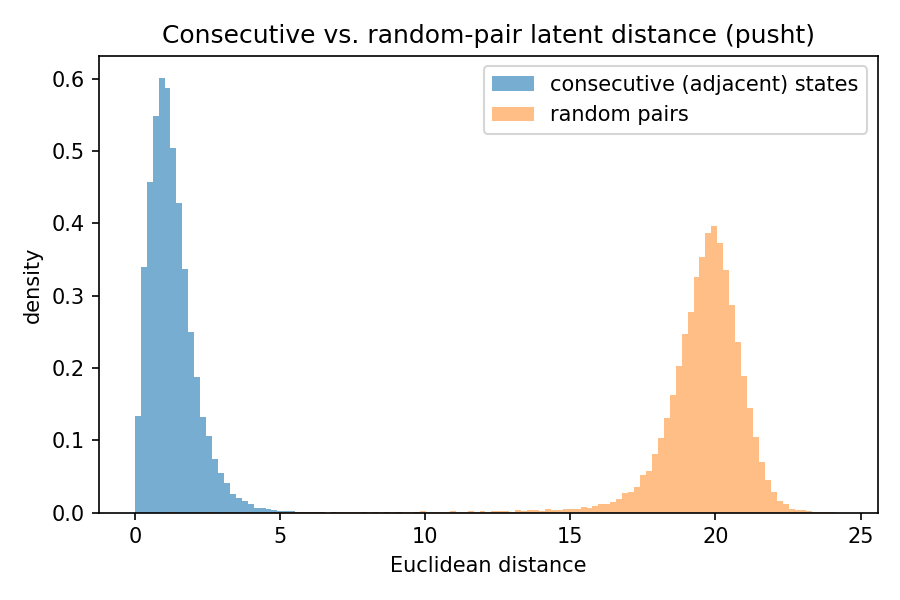
\includegraphics[width=0.75\linewidth]{figures/pusht_adjacent_vs_random.png}
\caption{Consecutive states sit at mean $1.28$ (median $1.15$), a full order of magnitude
below Two-Room's $11.75$. Random pairs are comparable to Two-Room's ($19.57$ vs.\ $19.25$) ---
so the gap between ``one real step'' and ``two arbitrary states'' is far larger in Push-T's
embedding than in Two-Room's. This alone is a strong hint that Push-T's dynamics move the
encoder's output much more slowly per step, consistent with slow, continuous contact
manipulation rather than Two-Room's larger free-space steps.}
\label{fig:pusht-adjacent-vs-random}
\end{figure}

\begin{figure}[H]
\centering
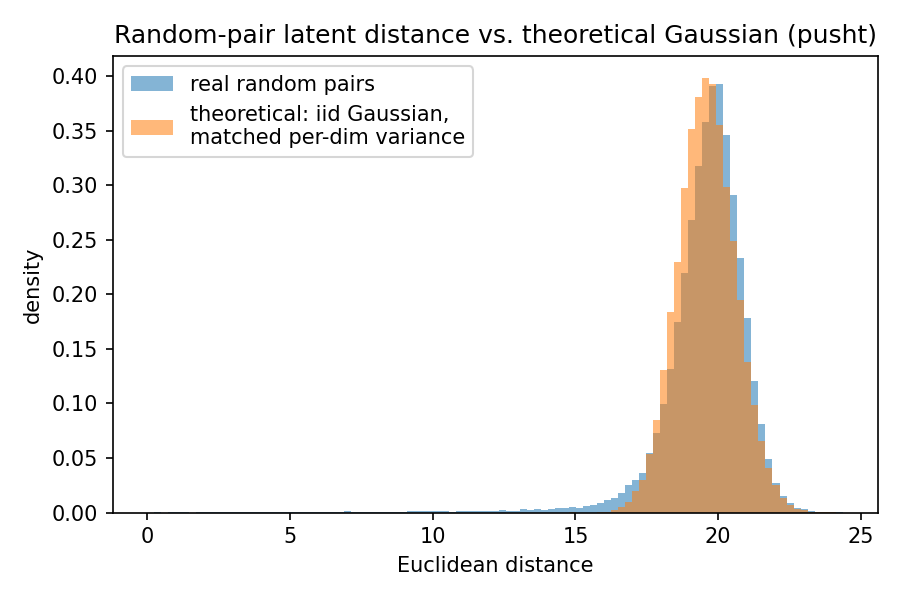
\includegraphics[width=0.75\linewidth]{figures/pusht_random_vs_theoretical.png}
\caption{Real random-pair distances (mean $19.57$) closely track the theoretical
matched-variance Gaussian reference (mean $19.60$) --- as close a match as Two-Room's
($19.25$ vs.\ $19.32$). At the level of pairwise distance statistics alone, Push-T's
embedding looks just as Gaussian-like in aggregate as Two-Room's; whatever breaks
\texttt{main.tex}'s calibration formula on Push-T, it is not visible in this particular
statistic.}
\label{fig:pusht-random-vs-theoretical}
\end{figure}

\textbf{Correction (6 September 2026): the four items below replace an earlier, wrong
analysis.} The original version of this section fed the predictor a single real action,
zero-padded into the 10-dim slot $\mathrm{action\_encoder}$ expects, and compared its output
one real step later -- and found what looked like a predictor performing at roughly chance
level. That invocation was wrong, not the model. The checkpoint's actual training convention
(\texttt{docs/lewm.txt}, Appendix D) applies a \textbf{frame-skip of 5}: one predictor call
consumes the concatenation of \textbf{5 consecutive real actions} ($5\times2{=}10$ dims,
exactly matching $\mathrm{action\_encoder}$'s input size with no padding at all) and
predicts the state \textbf{5 real steps} later, not 1. Three specific bugs were ruled out
before this deeper one was found -- wrong action-encoder slot (all $10$ zero-padding
positions land in the same narrow MSE band), the action pathway being ignored (predictions
do vary with different real actions), and off-by-one frame/action alignment
(\texttt{action[i]} genuinely beats \texttt{action[j]}) -- see
\texttt{[[lewm-action-encoder-padding]]} in memory for that record. None of those three was
the actual explanation; the block-size mismatch was.

\textbf{Second correction (9 September 2026): the 6 September numbers above were themselves
still wrong.} The block-size fix was correct, but the actions feeding
$\mathrm{action\_encoder}$ were still \emph{raw}, not z-scored. The checkpoint consumes
z-scored actions on both sides of the pipeline (\texttt{train.py}'s column normalizer,
\texttt{eval.py}'s \texttt{StandardScaler}) -- see \texttt{CLAUDE.md}, ``Action
normalization,'' and the companion correction in \texttt{latent-horizon-pusht.tex}. Push-T's
action std is $\approx 0.206$, so raw actions are $\mathbf{4.82\times}$ too small, which
reads to the predictor as a near-stationary command -- exactly the ``flat, no history
benefit, but otherwise unremarkable'' picture the 6 September numbers showed. Figures
\ref{fig:pusht-predictor-history}--\ref{fig:pusht-splice-verification} below are regenerated
with z-scored actions (\texttt{scripts/latent\_diagnostics.py env=pusht}, action stats
computed over the full dataset action column, same convention as \texttt{idm\_gate.py}); the
6 September values they replace are kept in the running text below for comparison, labeled
as such.

\begin{figure}[H]
\centering
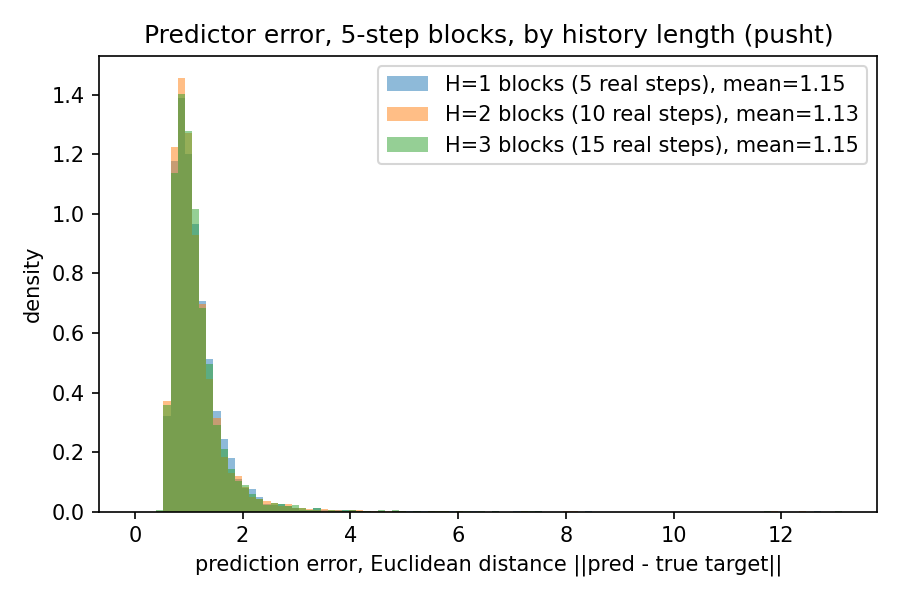
\includegraphics[width=0.75\linewidth]{figures/pusht_predictor_error_by_history.png}
\caption{Predictor error with z-scored actions (5-action-block convention, corrected 9
September), at $H{=}1,2,3$ blocks of history ($5,10,15$ real steps of context), on 5000 real
chains per length: mean $1.152$, $1.133$, $1.149$ (median $1.025$, $0.996$, $1.012$; q90
$1.675$, $1.631$, $1.662$). Error is still flat across $H$ -- still no benefit from Push-T's
documented history length of $3$ on this metric, the one genuine surprise that survives both
corrections. But the 6 September (raw-action) draft reported means $4.27$, $4.36$, $4.42$ --
roughly $3.7\times$ larger, and close to the raw 5-step real-movement scale itself
(\cref{fig:pusht-adjacent-vs-random} scaled up), i.e.\ a near no-motion error. With actions
correctly normalized, mean error $1.152$ sits right at the real single-step movement scale
($1.15$), not at the movement scale of the whole 5-step block -- the predictor is now
explaining most of a block's real displacement, not almost none of it.}
\label{fig:pusht-predictor-history}
\end{figure}

\begin{figure}[H]
\centering
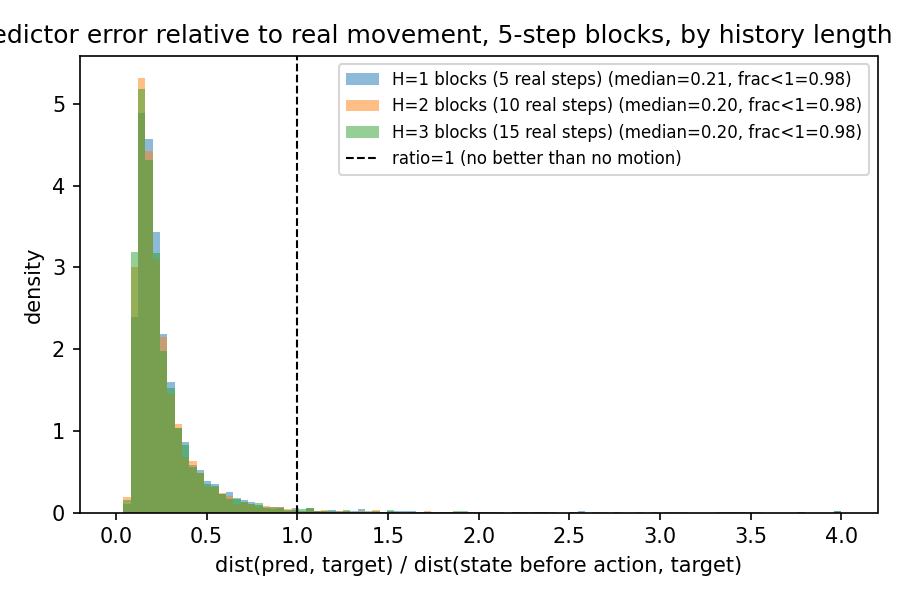
\includegraphics[width=0.75\linewidth]{figures/pusht_predictor_ratio_by_history.png}
\caption{The same comparison, normalized: $\mathrm{dist}(\mathrm{pred},\mathrm{target}) /
\mathrm{dist}(\mathrm{state\ before\ the\ block},\mathrm{target})$. With z-scored actions,
median ratio $\approx 0.20$ at every $H$ ($0.206$, $0.195$, $0.197$), $98\%$ of blocks
showing improvement over no motion ($97.8\%$, $98.3\%$, $98.0\%$), and $\sim\!91\%$ landing
below half the no-motion error. The 6 September (raw-action) draft reported median
$\approx 0.78$ at every $H$ -- real signal, but far weaker than this. Push-T's predictor
carries substantial one-block predictive signal, considerably more than either the original
zero-padded invocation (roughly chance level) or the block-size-fixed-but-unnormalized draft
suggested.}
\label{fig:pusht-predictor-ratio}
\end{figure}

\begin{figure}[H]
\centering
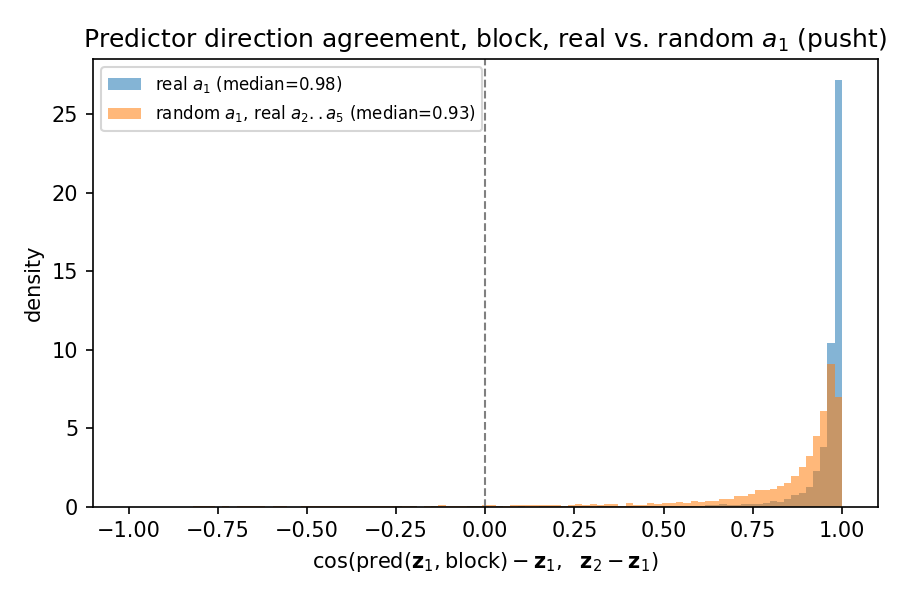
\includegraphics[width=0.75\linewidth]{figures/pusht_predictor_direction_agreement.png}
\caption{Direction agreement on a real one-block ($H{=}1$, 5-real-step) transition, with a
control, z-scored actions: real $a_1$ gives mean $0.955$, median $0.982$, $99.1\%$ above
$0.5$ -- near-ceiling, and a further large upward revision from the 6 September (raw-action)
draft (mean $0.748$, median $0.800$, $90.5\%$ above $0.5$), which was itself a large revision
from the original zero-padded draft (mean $0.489$, median $0.534$). Replacing $a_1$ with a
random real action while keeping $a_2,\dots,a_5$ real drops this to mean $0.842$, median
$0.929$, $92.7\%$ above $0.5$ --- a gap of $0.053$ in median cosine (6 September: $0.074$),
versus Two-Room's $0.302$ drop under the identical control (\texttt{latent-diagnostics.tex},
unaffected by this bug -- Two-Room's raw actions were only $1.15\times$ off, not
$4.82\times$). Push-T's one-block direction is still driven much more by the last four real
actions than by the first, consistent with its rate-limited, positional-goal action
semantics. \textbf{This remains a real caveat on \cref{fig:pusht-splice-verification}'s
result}: even with both bugs fixed, the real-vs-random direction gap stays small relative to
Two-Room's, so this particular test is a comparatively weak probe of whether the IDM's
specific inferred action is good -- ``almost any $a_1$'' still scores respectably here.
\cref{fig:pusht-splice-verification}'s own result, however, no longer agrees with that
caveat as cleanly as the 6 September draft implied -- see its caption.}
\label{fig:pusht-predictor-direction}
\end{figure}

\begin{figure}[H]
\centering
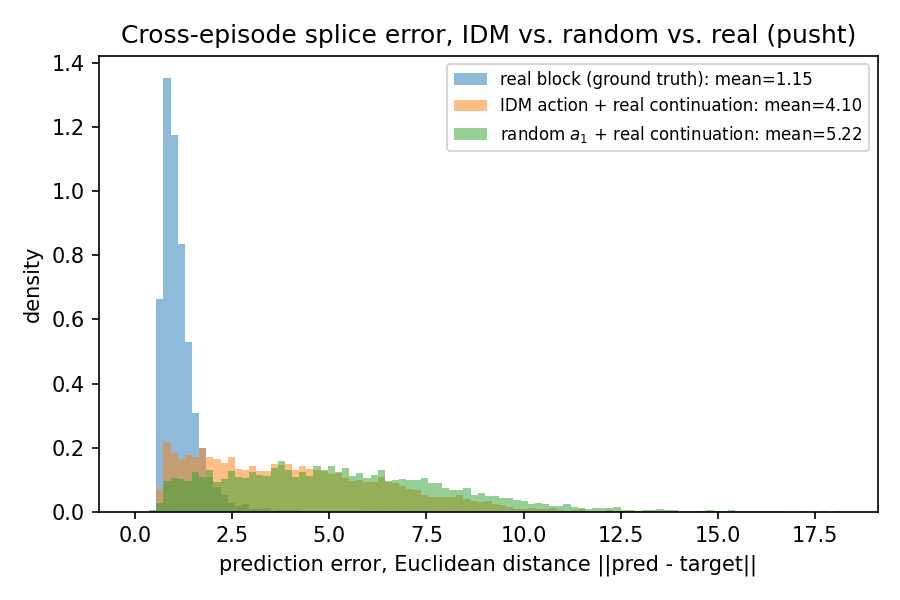
\includegraphics[width=0.75\linewidth]{figures/pusht_splice_vs_ground_truth.png}
\caption{The test this correction was actually for, now with the same random-$a_1$ control
as \cref{fig:pusht-predictor-direction}, z-scored actions throughout (including the IDM
ensemble's own training data): does an IDM-inferred connecting action, for a candidate
cross-episode pair $(\zv_i,\zv_j)$ from the wide top-20 pool, do \emph{better} than an
uninformed guess? Three conditions predicting from $\zv_i$ against $\zv_{j+4}$: the IDM
hybrid block $(a,\ a_j,\ a_{j+1},\ a_{j+2},\ a_{j+3})$; the same block with $a$ replaced by a
random real action; and the reference (\cref{fig:pusht-predictor-history}'s $H{=}1$ real
block error). Result: IDM hybrid mean $4.103$, median $3.748$ (ratio to no-motion baseline:
median $0.645$, $79.7\%$ below $1$); random-$a_1$ control mean $5.221$, median $4.951$
(ratio median $0.811$, $68.9\%$ below $1$); real reference mean $1.152$, median $1.025$.
\textbf{The IDM-vs-random gap is no longer small}: median $3.748$ vs.\ $4.951$, the IDM
hybrid error is about $24\%$ lower -- a real reversal of the 6 September (raw-action) draft's
finding of a $\approx\!4\%$ gap ($5.37$ vs.\ $5.59$). The IDM's specific inference does earn
its keep here, just not to Two-Room's degree (roughly $2\times$ separation there) --- and the
hybrid block is still $\sim\!3.7\times$ worse than a genuine in-episode block (median $3.748$
vs.\ $1.025$), so cross-episode splicing remains far harder than real, in-distribution
prediction. Read together with \cref{fig:pusht-predictor-direction}'s comparatively small
real-vs-random \emph{direction} gap, the two tests now disagree in degree (large gap here,
small gap there) though not in direction -- both still favor the real/IDM condition over
random. \cref{fig:pusht-predictor-direction}'s caveat about this being a structurally weaker
probe on Push-T than on Two-Room still holds; it no longer implies the IDM's inference adds
\emph{nothing} measurable in the splice setting.}
\label{fig:pusht-splice-verification}
\end{figure}

\begin{figure}[H]
\centering
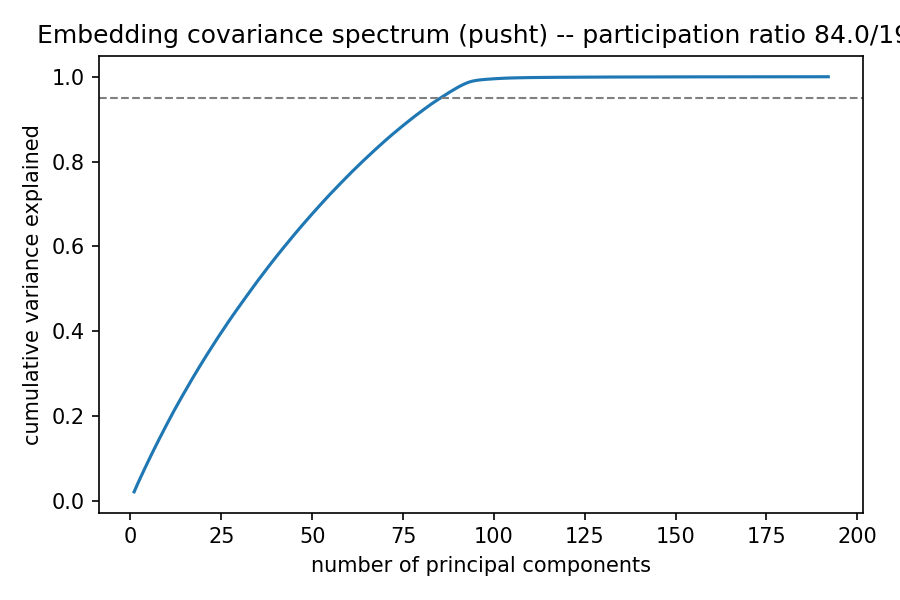
\includegraphics[width=0.75\linewidth]{figures/pusht_pca_spectrum.png}
\caption{Participation ratio $83.95$ of $192$ ambient dimensions --- almost exactly matching
\texttt{main.tex}'s own previously-reported Push-T figure ($84$ of $192$), a useful
consistency check that this independently-built script reproduces established numbers. Also
close to Two-Room's $86.36$, continuing that document's point: effective dimensionality alone
does not predict which environment's calibration formula holds.}
\label{fig:pusht-pca-spectrum}
\end{figure}

\begin{figure}[H]
\centering
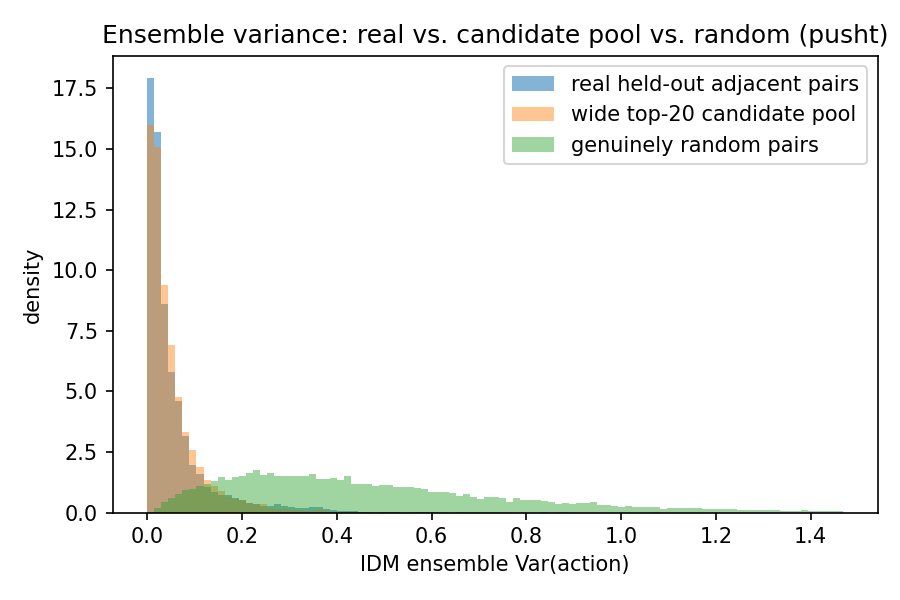
\includegraphics[width=0.75\linewidth]{figures/pusht_idm_variance_comparison.png}
\caption{IDM ensemble variance: real transitions $0.00267$, the wide top-20 candidate pool
$0.00282$ (nearly identical, as on Two-Room), genuinely random pairs $0.0284$ --- again an
order of magnitude higher. The qualitative story is identical to Two-Room's: variance
separates ``connectable'' from ``genuinely unrelated'' cleanly, it simply has little left to
discriminate within an already-mostly-connectable candidate pool. Absolute values are smaller
throughout, consistent with Push-T's smaller action/movement scale overall
(\cref{fig:pusht-adjacent-vs-random}).}
\label{fig:pusht-idm-variance}
\end{figure}

\begin{figure}[H]
\centering
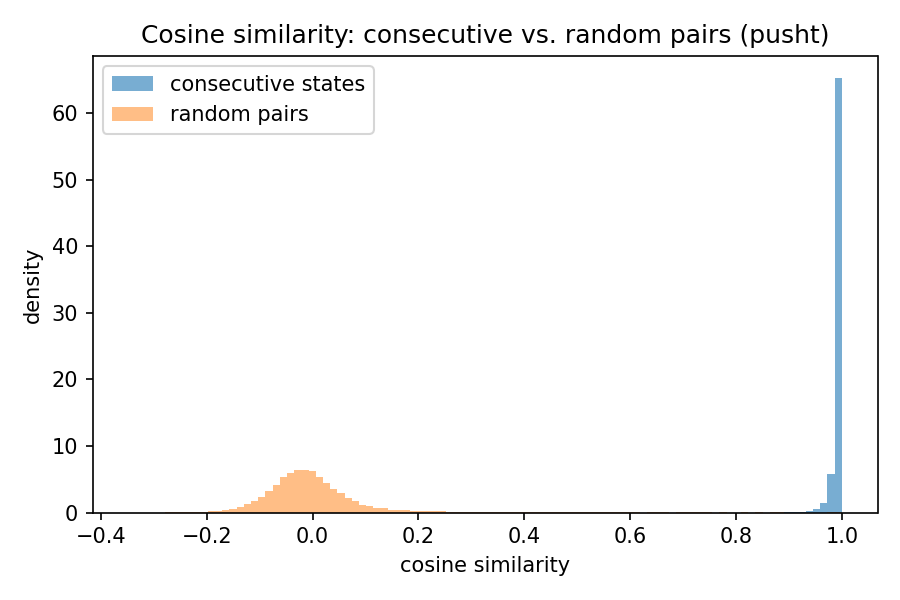
\includegraphics[width=0.75\linewidth]{figures/pusht_cosine_similarity.png}
\caption{Cosine similarity: consecutive states $0.9938$, random pairs $0.0036$. This is the
figure where Push-T and Two-Room diverge most sharply --- Two-Room's adjacent-pair cosine is
$0.540$, not $0.99$. A same-episode consecutive pair in Push-T is very nearly the same vector.
This is the direct geometric picture behind \texttt{main.tex}'s diagnosis of why the
calibration formula fails on Push-T ($\hat\rho$ statistically $\ge 1$): $\hat\rho$ is
essentially this same one-step correlation number, and a cosine this close to $1$ pushes
$\varepsilon^2 = 2(1-\hat\rho)F^{-1}_{\chi^2_d}(q)$ toward zero (or negative under estimation
noise) by construction, independent of any deeper representational problem.}
\label{fig:pusht-cosine-similarity}
\end{figure}

\textbf{Summary: where Push-T matches Two-Room, and where it genuinely does not.}
\begin{itemize}[leftmargin=1.4em,itemsep=2pt]
\item \textbf{Matches:} the random-vs-theoretical-Gaussian fit
(\cref{fig:pusht-random-vs-theoretical}), the PCA participation ratio
(\cref{fig:pusht-pca-spectrum}), and the qualitative variance-separates-connectable-from-random
story (\cref{fig:pusht-idm-variance}) all look like Two-Room's, sometimes to within a couple
of percent. None of these predict the calibration failure on their own.
\item \textbf{Differs, and matters:} adjacent-pair scale is $9\times$ smaller
(\cref{fig:pusht-adjacent-vs-random}), and adjacent-pair cosine is nearly $1$ instead of
$0.54$ (\cref{fig:pusht-cosine-similarity} -- this is the number that actually explains the
calibration failure). The predictor itself is \emph{not} markedly weaker once invoked
correctly (\cref{fig:pusht-predictor-history,fig:pusht-predictor-direction}) -- that was an
invocation bug in the original version of this document, not a property of Push-T. There is
a real, smaller gap left after the correction: Push-T's predictor is somewhat less reliable
than Two-Room's on both magnitude and direction, and (with the random-$a_1$ control added)
the IDM's specific inference produces only a small edge over a random action on the
cross-episode splice test ($4\%$ gap vs.\ Two-Room's $\sim\!2\times$), consistent with the
same small gap in the direction-agreement control.
\item \textbf{Practical implication for any future Push-T work on the E2 line}
(\texttt{predictor-stitching.tex}): the predictor itself is not broken here (the corrected
figures show real one-block signal), but the two random-action controls together show the
IDM-ensemble's SPECIFIC contribution is weak on Push-T's cross-episode setting --- most of
what makes the hybrid block better than nothing comes from $j$'s own real continuation
actions, not from what the IDM inferred. This is a materially more cautious conclusion than
the single-condition splice result suggested: an E2-style acceptance criterion for Push-T
should not assume the IDM's inference is doing the identification work it clearly does on
Two-Room, and the mechanism may need a genuinely different design here, not just more slack
on the same one.
\end{itemize}

\section{Pred1: a genuinely-trained 1-step predictor}
\label{sec:pred1}

Everything above uses \texttt{quentinll/lewm-pusht}'s pretrained predictor under its real
5-action-block, frame-skip-5 training convention (call this \textbf{block5}). This section
covers a second, separately-trained checkpoint,
\texttt{data/checkpoints/lewm\_pusht\_1step\_predictor} (\texttt{weights\_epoch\_20.pt}),
hereafter \textbf{pred1}: the same frozen \texttt{quentinll/lewm-pusht} encoder (so landmark
embeddings $\zv$ are identical to block5's) feeding a small \texttt{ARPredictor}
(depth $2$, hidden dim $96$) plus a fresh \texttt{action\_encoder} with \texttt{input\_dim=2}
-- no block concatenation, no padding -- trained from scratch for $20$ epochs directly on real
$(\zv_t, a_t) \to \zv_{t+1}$ triples (\texttt{config/train/lewm\_pusht\_1step.yaml}). It has
\texttt{num\_frames=1}: it only ever accepts single-frame context, by design.

\textbf{Every statistic in this section is a genuine single real step: one real action in,
one real next state out.} \texttt{scripts/latent\_diagnostics.py predictor=1step} runs with
\texttt{SKIP=1} throughout, so the direction-agreement and splice-verification tests below do
\emph{not} splice in a 4-real-action continuation the way the block5 figures above do -- there
is no continuation to ignore or include, because a single pred1 call already \emph{is} the
whole test. Figures use a \texttt{pusht1step\_} prefix to keep them separate from block5's.

\begin{figure}[H]
\centering
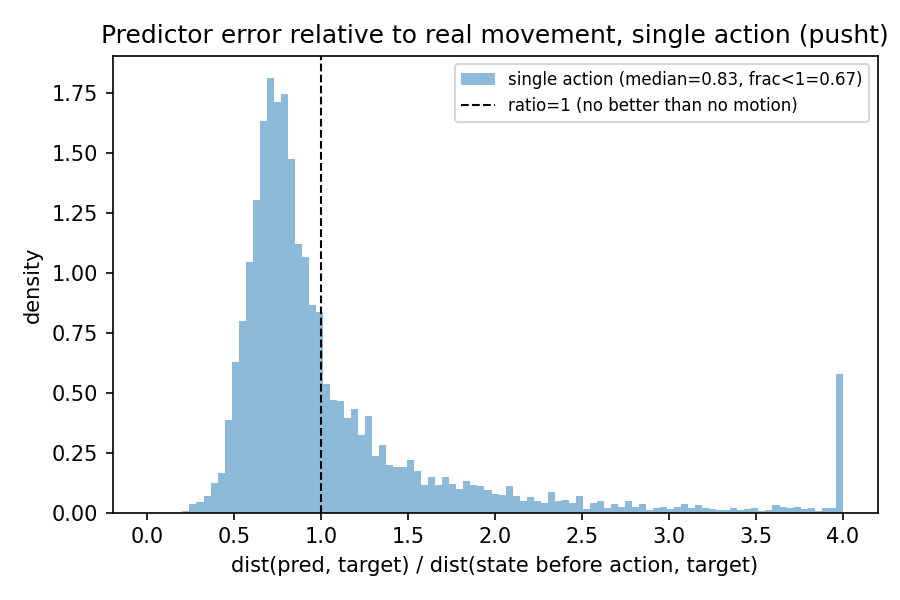
\includegraphics[width=0.75\linewidth]{figures/pusht1step_predictor_ratio_by_history.png}
\caption{Real single-step accuracy: mean error $1.092$, median $0.980$ -- right at the scale
of a real step itself (\cref{fig:pusht-adjacent-vs-random}'s median $1.15$), not block5's
$\sim\!4$--$5$ (a different, larger, 5-real-step scale, not a worse predictor). Ratio
$\mathrm{dist}(\mathrm{pred},\mathrm{target})/\mathrm{dist}(\mathrm{before},\mathrm{target})$:
median $0.832$, $67.4\%$ of steps show \emph{some} improvement over assuming no motion. A
genuinely useful, well-behaved 1-step predictor on its own terms.}
\label{fig:pusht1step-ratio}
\end{figure}

\begin{figure}[H]
\centering
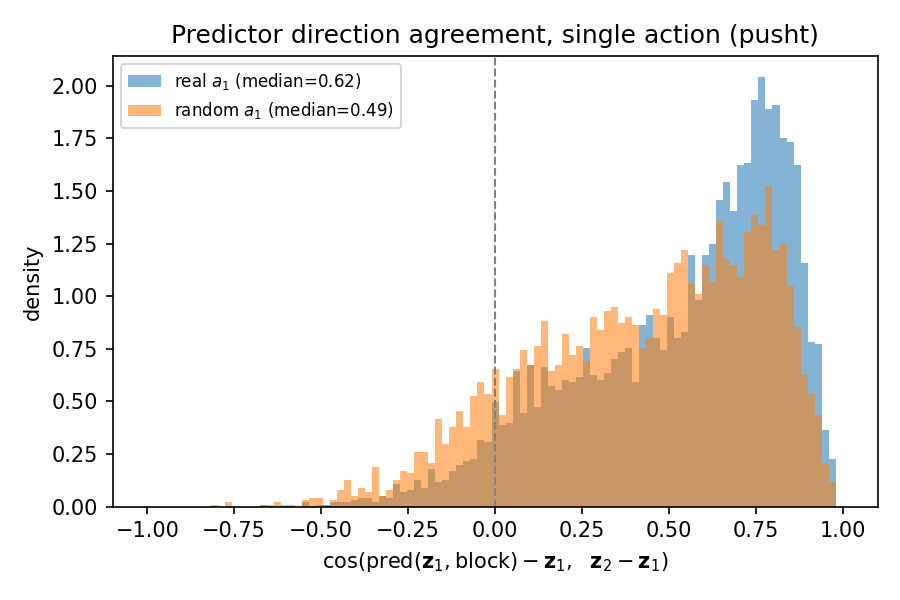
\includegraphics[width=0.75\linewidth]{figures/pusht1step_predictor_direction_agreement.png}
\caption{Direction agreement on a bare single real action (no continuation at all): real
$a_1$ gives mean $0.537$, median $0.622$. Replacing it with a random real action drops this to
mean $0.430$, median $0.487$ -- a $0.135$ drop in median cosine. This is a real,
meaningful gap (almost double block5's $0.074$ drop under the same control), consistent with
pred1 actually depending on the single action it is given, rather than most of its signal
riding on continuation actions it does not even receive.}
\label{fig:pusht1step-direction}
\end{figure}

\begin{figure}[H]
\centering
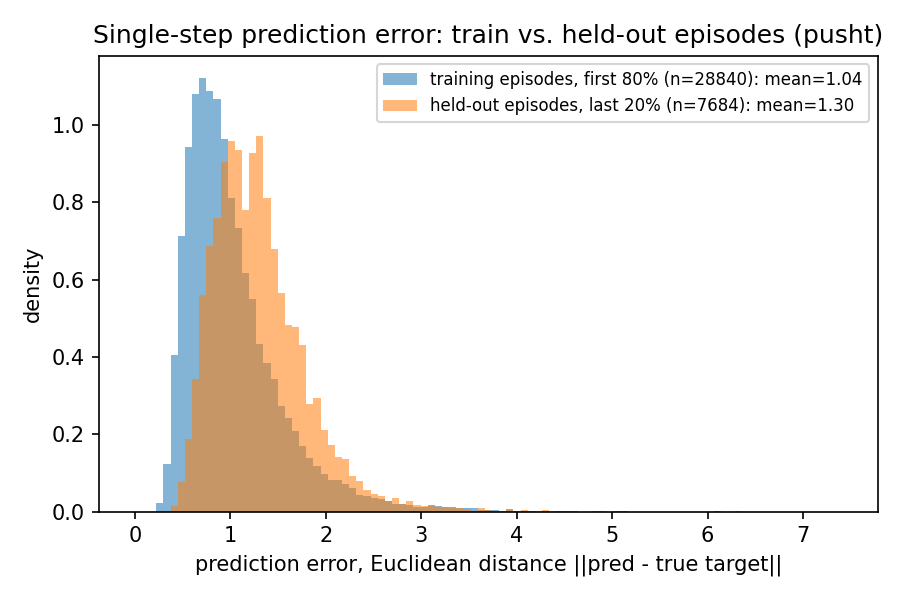
\includegraphics[width=0.75\linewidth]{figures/pusht1step_predictor_error_train_vs_test.png}
\caption{Does pred1's real single-step accuracy hold up on episodes it never trained on?
Split by the same convention pred1 was actually trained under
(\texttt{config/train/lewm\_pusht\_1step.yaml}: contiguous $80/20$ split, first $80\%$ of
episodes on-disk order for train, last $20\%$ held out) -- not the random episode shuffle
used elsewhere in this script for the IDM ensemble. Training episodes: $n{=}28{,}840$, mean
$1.036$, median $0.907$. Held-out (last $20\%$) episodes: $n{=}7{,}684$, mean $1.305$, median
$1.236$ -- about $36\%$ higher. A real but modest generalization gap: pred1 is measurably
worse on truly unseen episodes, consistent with only $20$ epochs of training on a small model,
but the held-out error is still an order of magnitude below the $\approx\!4.3$-unit
candidate-pool gap in \cref{fig:pusht1step-splice} below -- this gap does not explain that
figure's negative result.}
\label{fig:pusht1step-train-test}
\end{figure}

\begin{figure}[H]
\centering
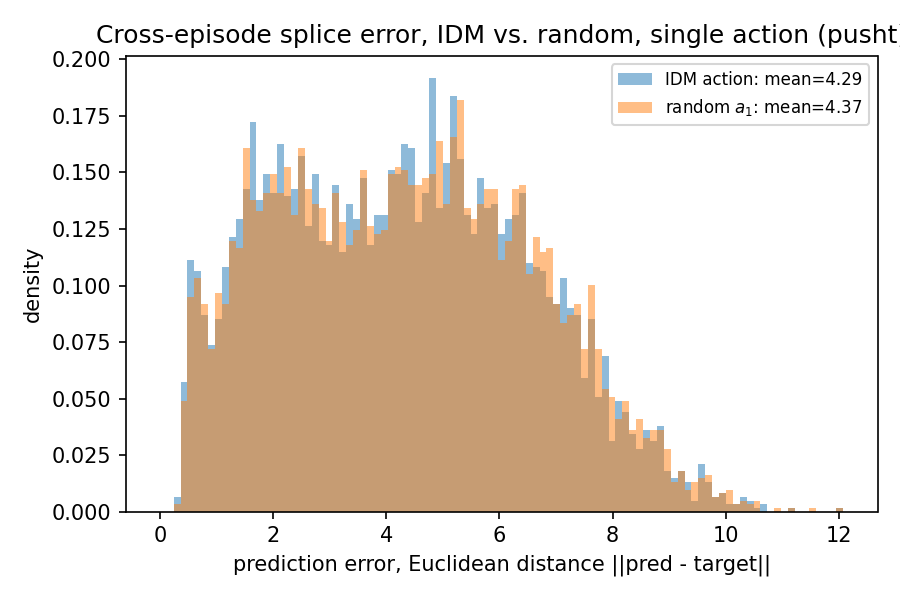
\includegraphics[width=0.75\linewidth]{figures/pusht1step_splice_vs_ground_truth.png}
\caption{Single-step splice test, IDM vs.\ random action only (the real-reference comparison
now has its own dedicated figure above): for a candidate cross-episode pair $(\zv_i,\zv_j)$
from the same wide top-20 pool used throughout, does $\mathrm{pred1}(\zv_i, a)$ land near
$\zv_j$ \emph{itself} (no intermediate hops) for the IDM-inferred $a$, versus a random real
action? Result: IDM hybrid mean $4.293$, median $4.271$; random-$a_1$ control mean $4.368$,
median $4.345$ -- statistically indistinguishable (ratio medians $1.007$ vs.\ $1.024$), a
similar negative verdict to block5's. \textbf{The cause is different here, and diagnosable
directly from these numbers}: the candidate pool's own starting gap
$\mathrm{dist}(\zv_i,\zv_j)$ is $\approx 4.3$ (visible as the hybrid/random error itself,
since ratio $\approx 1$) -- almost $4\times$ larger than a real single step's $1.15$-unit
reach (\cref{fig:pusht-adjacent-vs-random}), and well beyond even the held-out generalization
error in \cref{fig:pusht1step-train-test} above. No single action, real, random, or
IDM-inferred, can close a $4.3$-unit gap in one step, because pred1's own dynamics do not move
that far per call. This is not a defect in pred1 or in the IDM: it is the top-20 kNN candidate
pool sitting at a distance scale built for block5's much larger per-call reach, not pred1's.}
\label{fig:pusht1step-splice}
\end{figure}

\begin{figure}[H]
\centering
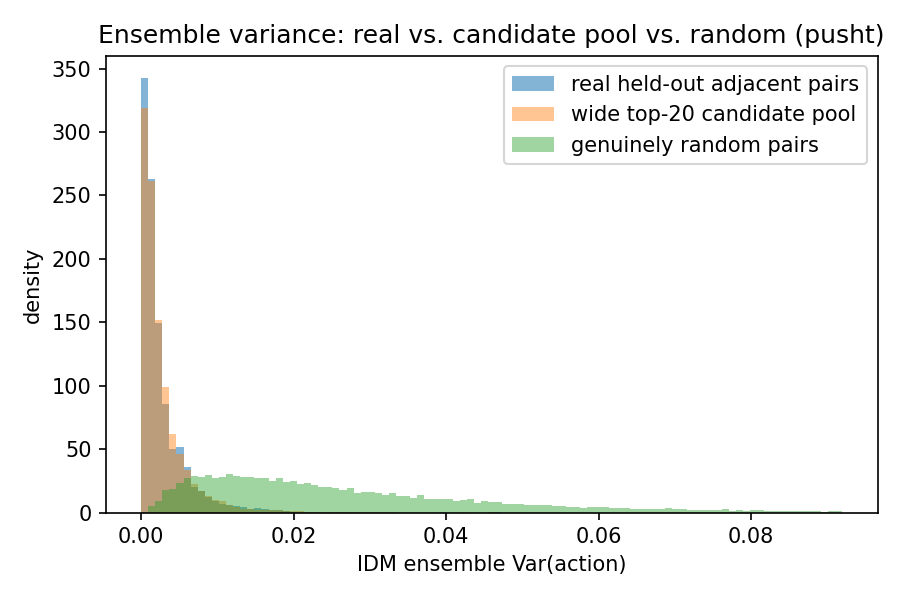
\includegraphics[width=0.75\linewidth]{figures/pusht1step_idm_variance_comparison.png}
\caption{IDM ensemble variance under pred1's landmark set: real held-out transitions
$0.00267$, the wide top-20 candidate pool $0.00282$ (indistinguishable from real, same
pattern as block5), genuinely random pairs $0.0284$ ($\sim\!10\times$ higher). Consistent
with \cref{fig:pusht1step-splice}: the candidate pool looks statistically like real
transitions to the IDM, it is simply too far away for a single pred1 step to verify by
prediction error alone.}
\label{fig:pusht1step-variance}
\end{figure}

\begin{figure}[H]
\centering
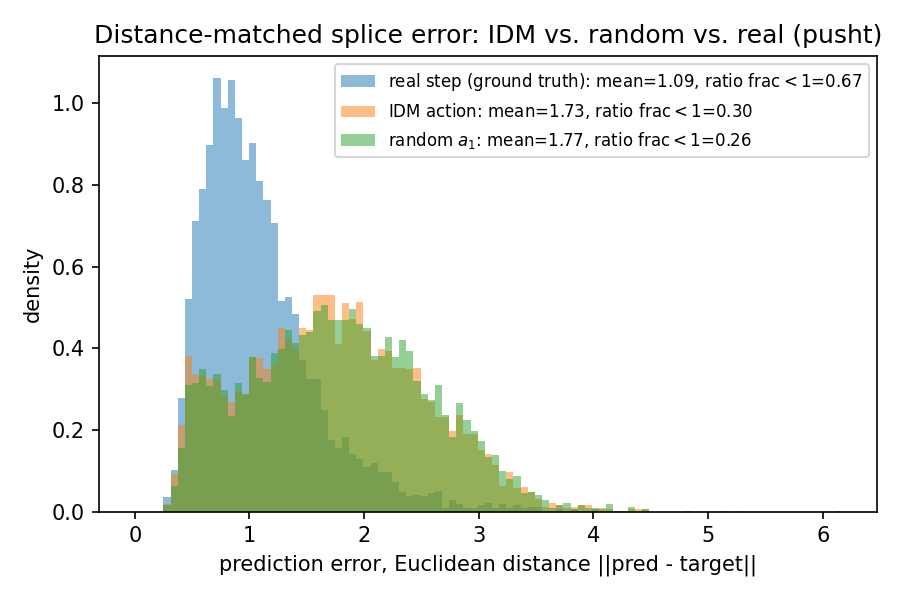
\includegraphics[width=0.75\linewidth]{figures/pusht1step_splice_distance_filtered.png}
\caption{Direct test of the distance-scale hypothesis raised by \cref{fig:pusht1step-splice}:
rebuild the candidate pool restricted to a distance pred1 can actually cover -- radius
$=2.735$, the $95$th percentile of the REAL adjacent-step distance
(\cref{fig:pusht-adjacent-vs-random}), calibrated from data rather than an arbitrary constant
-- filtering the same bounded top-20 pool from $216{,}431$ down to $63{,}456$ pairs with mean
gap $1.500$ (median $1.577$), now directly comparable to a real step's $1.15$-unit median.
\textbf{The IDM-vs-random gap barely moves}: IDM error mean $1.729$ (median $1.703$), random
error mean $1.769$ (median $1.746$) -- still statistically indistinguishable.
\textbf{This rules out the distance-scale hypothesis as the (sole) explanation.} The more
revealing number is the fraction of pairs where prediction actually lands closer to the target
than the starting point (ratio $<1$): only $30.3\%$ for the IDM action and $26.0\%$ for random,
versus $67.4\%$ for real single steps at essentially the same distance scale
(\cref{fig:pusht1step-ratio}). At matched distance, real transitions and cross-episode
candidates behave qualitatively differently -- most real steps get closer under prediction,
most distance-matched candidates do not, for either action. This is evidence that these
candidates are mostly \emph{not} one real step apart to begin with: they are coincidentally
nearby in latent space (plausibly a state-space symmetry in Push-T's manipulation task, e.g.
different paths reaching a similar block configuration), with no real single action connecting
most of them -- which would also explain why no action, real or inferred, can be found that
closes the gap.}
\label{fig:pusht1step-distance-filtered}
\end{figure}

\textbf{Summary: pred1 is a better predictor than block5 was ever asked to be at this task,
and the splice test's failure is not a scale artifact -- it reflects a real property of the
candidate pool.} Pred1's own one-step accuracy and action-sensitivity are both good, and
clearly better-behaved than block5's under the equivalent single-real-action control
(\cref{fig:pusht1step-direction} vs.\ \cref{fig:pusht-predictor-direction}). The first
hypothesis for the splice test's failure -- that \texttt{raw\_topk\_cross\_episode\_pairs
(k=20)}'s candidates sit $\approx\!4\times$ farther apart than pred1's real per-step reach --
was directly testable, and confirmed: restricting to a distance-matched pool
(\cref{fig:pusht1step-distance-filtered}) does not recover an IDM-vs-random gap. Instead it
reveals the deeper issue: even at matched distance, most of these candidates are not real
one-step neighbors at all (only $\sim\!28\%$ improve under any action, vs.\ $67\%$ for real
steps) -- they are latent-space coincidences, not genuine transitions. \textbf{Practical
implication:} for Push-T, neither block5 nor pred1, at any candidate distance scale tried so
far, gives a working predictor-based identification-edge verifier. The existing plain-metric
k-capped kNN construction (already in production, see \texttt{main.tex}'s B0 gate) remains the
best available mechanism until a genuinely different verification signal is found -- adding an
IDM/predictor-based filter on top of it is not yet justified by any result in this document.

\section{Scaling the ensemble: confidence, capacity, and data}
\label{sec:scaling}

Section \ref{sec:pred1}'s distance-filtered result left one obvious follow-up unaddressed:
could the IDM ensemble itself be improved, rather than accepting the splice test as a dead
end? This section runs that question down through four increasingly targeted experiments --
selecting candidates by confidence, checking model capacity, checking training-data scale,
and finally re-running the full splice test against a properly-fixed ensemble -- on a smaller,
independent testbed (expert\_30: a random 30-episode Push-T landmark set, distinct from the
300-episode set used everywhere above) before scaling the winning fix to the full dataset.

\subsection{A cleaner testbed: expert\_30 with a calibrated distance threshold}

30 episodes (4{,}031 landmarks) were encoded fresh, and cross-episode candidates were built
by filtering a kNN search to distance $\le 5$ -- the user-specified upper bound on real
consecutive-state distance, close to this tier's own 99th-percentile real adjacent-step
distance ($3.639$; real adjacent stats: mean $1.256$, median $1.140$, max $6.739$). This
produced $1{,}718$ candidate pairs, mean gap $3.402$ (median $3.687$) -- still noticeably
larger than the real median, since genuinely close cross-episode neighbors are rare at this
small scale. The splice test on this pool reproduced the same qualitative result as
Section \ref{sec:pred1}'s: IDM error mean $3.537$/median $3.687$ (frac$<$1 $=0.362$) vs.\
random mean $3.572$/median $3.725$ (frac$<$1$=0.338$) vs.\ real reference mean $1.071$/median
$0.952$ (frac$<$1$=0.683$) -- IDM and random remain statistically indistinguishable on an
entirely independent landmark sample.

\subsection{Does ensemble confidence predict correctness?}
\label{sec:confidence}

The natural next question: even if the IDM's \emph{average} action is no better than random,
does its \emph{confidence} (inter-member variance) pick out the subset of candidates where it
\emph{is} right? Two tests, both negative in the specific way that matters:

\textbf{Selecting by confidence changes the absolute rate, not the IDM's edge over random.}
Ranking the $1{,}718$ candidates by ascending ensemble variance and restricting to
progressively smaller, more-confident subsets:

\begin{center}
\begin{tabular}{@{}lrrrr@{}}
\toprule
top-$X\%$ by confidence & $n$ & IDM frac$<$1 & random frac$<$1 & gap (pts) \\
\midrule
100\% & 1718 & 0.362 & 0.338 & 2.4 \\
50\%  & 859  & 0.433 & 0.424 & 0.9 \\
25\%  & 429  & 0.527 & 0.513 & 1.4 \\
10\%  & 171  & 0.526 & 0.515 & 1.1 \\
5\%   & 85   & 0.529 & 0.506 & 2.3 \\
\bottomrule
\end{tabular}
\end{center}

Confident candidates \emph{are} more plausible overall -- frac$<$1 rises from $36\%$ toward
$\sim\!53\%$, closer to the real reference's $68\%$ -- but the IDM-vs-random gap stays flat
at every confidence level (never above $\sim$2.4 points). Low variance tracks ``this pair is
probably connectable by \emph{some} action,'' not ``the IDM's specific action is correct.''

\begin{figure}[H]
\centering
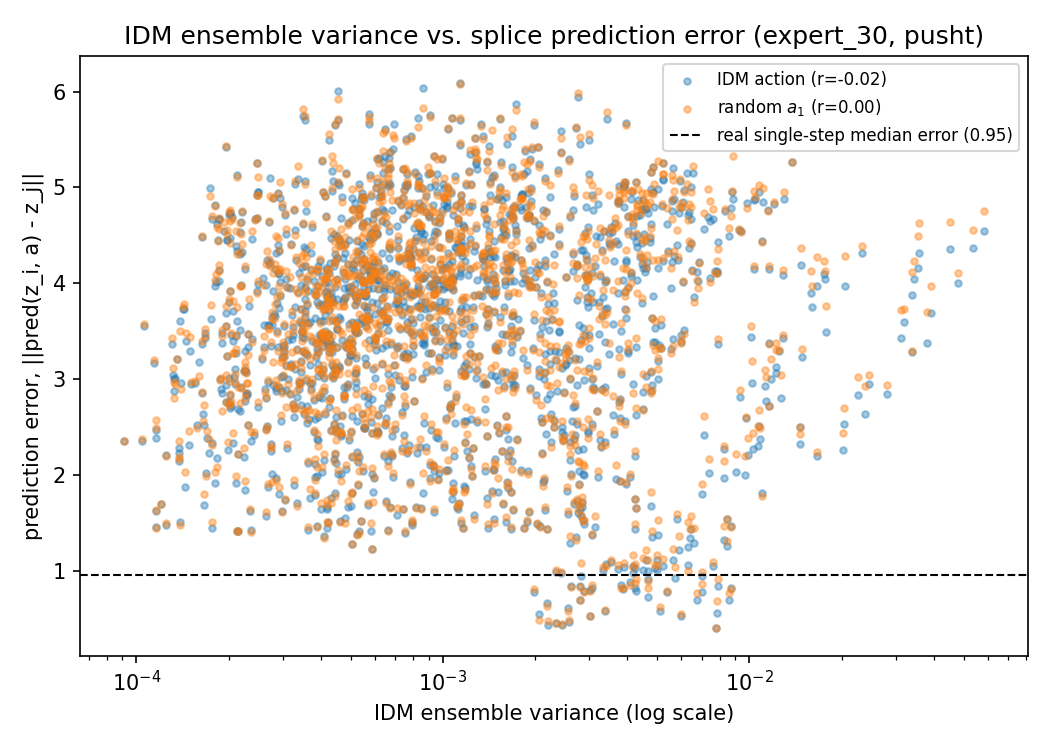
\includegraphics[width=0.75\linewidth]{figures/pusht_expert30_idmvar_vs_error.png}
\caption{IDM ensemble variance vs.\ splice prediction error, for both the IDM's inferred
action and a random control, on the same $1{,}718$ candidates. Pearson correlation:
$-0.018$ (IDM), $0.004$ (random) -- both indistinguishable from zero. The two series overlap
almost completely across the full variance range; there is no down-left-sloping cloud that
would indicate variance predicts error.}
\label{fig:expert30-idmvar-scatter}
\end{figure}

\textbf{A purpose-built discriminative classifier does no better -- and its confident
predictions are actively counterproductive.} Rather than relying on an action-regression
ensemble's incidental variance, a small classifier ensemble was trained to directly answer
``is this a real transition?'', using distance-matched negatives (for each real positive
transition, the nearest-distance cross-episode pair from a held-out pool, mean match error
$0.009$) so it could not simply learn ``small distance $=$ real.'' Sanity check: it separates
held-out real transitions (mean $P(\text{real})=0.966$) from genuinely random pairs (mean
$0.618$) only weakly. On the actual candidate pool, correlation with splice error is again
near zero ($0.027$ IDM, $0.021$ random) -- and selecting the classifier's \emph{most
confident} ``real'' candidates makes frac$<$1 \emph{worse}, not better ($36\%\to25\%\to21\%\to
7\%\to9\%$ from top-100\% to top-5\%). Whatever feature the classifier keys on to call a pair
``real,'' it is anti-correlated with actual one-step predictability -- a genuinely bad sign,
not just a null result.

\begin{figure}[H]
\centering
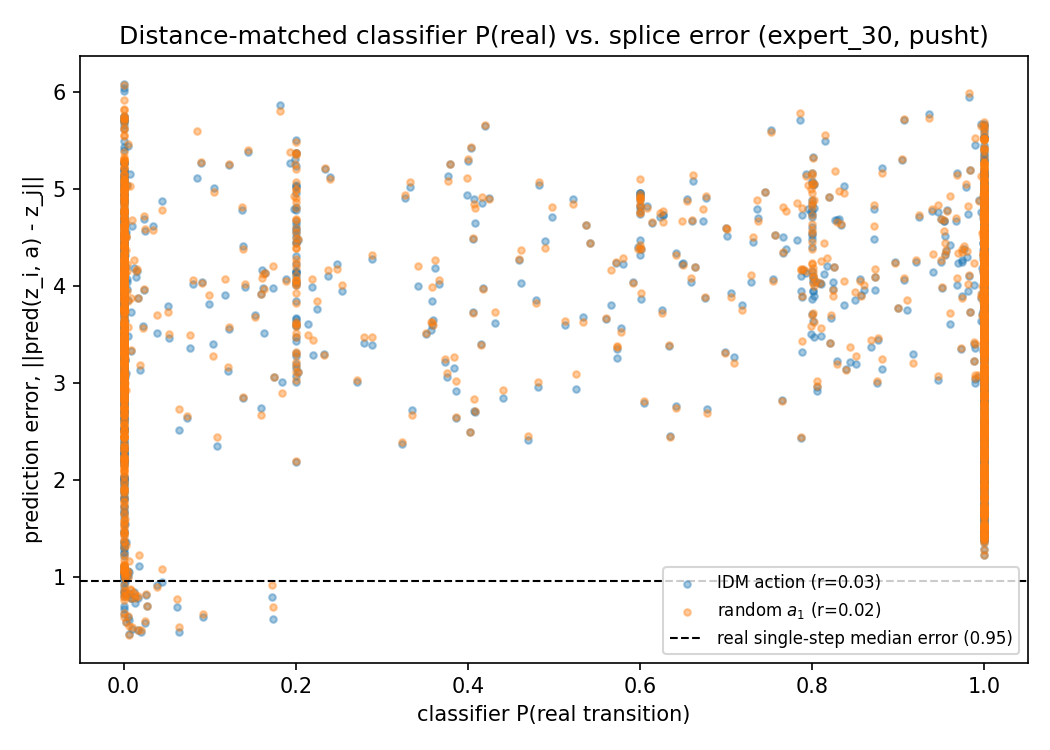
\includegraphics[width=0.75\linewidth]{figures/pusht_expert30_classifier_vs_error.png}
\caption{Distance-matched classifier $P(\text{real})$ vs.\ splice prediction error. No
downward trend for either the IDM action or the random control -- consistent with the
bucketed result showing classifier confidence actively anti-correlated with actual
performance at the tails.}
\label{fig:expert30-classifier-scatter}
\end{figure}

\subsection{Is the ensemble capacity-limited?}
\label{sec:capacity}

The natural hypothesis after two confidence signals failed: maybe the ensemble itself is too
small to represent Push-T's inverse dynamics, and a bigger MLP would fix everything. Tested
directly at expert\_30 scale (3{,}241 training pairs) by comparing hidden-layer width against
the held-out real action-recovery MSE reduction over a marginal (mean-training-action)
baseline -- the same metric used to validate the IDM ensemble in the very first sanity check
of this investigation (Two-Room E1):

\begin{center}
\begin{tabular}{@{}lrr@{}}
\toprule
hidden width & held-out MSE & reduction vs.\ marginal \\
\midrule
256  & 0.04055 & $-6.2\%$ \\
512  & 0.04777 & $-25.1\%$ \\
1024 & 0.04586 & $-20.1\%$ \\
\bottomrule
\end{tabular}
\end{center}

Every size tested performs \emph{worse} than the trivial baseline, and bigger is worse still
-- the classic signature of overfitting a small dataset, not underfitting. This directly rules
out ``make the MLP bigger'' as a fix: at this data scale, more capacity has nothing to fit
\emph{to} and only memorizes noise more precisely.

\subsection{The real bottleneck: training data scale}
\label{sec:datascale}

If capacity was never the problem, the natural remaining candidate is data volume. Push-T's
full dataset is $18{,}685$ episodes ($2{,}336{,}736$ frames) -- expert\_30's $3{,}241$ training
pairs and even Section \ref{sec:pred1}'s $29{,}461$-pair 300-episode set are a tiny fraction of
it. Using the precomputed frozen-encoder embeddings already produced for pred1's own training
(\texttt{pusht\_expert\_train\_emb.h5}, avoiding a re-encode of 2.3M raw-pixel frames), with a
\emph{fixed} $2{,}000$-episode held-out validation set used at every scale for direct
comparability:

\begin{center}
\begin{tabular}{@{}lrrr@{}}
\toprule
training pairs & episodes & held-out MSE reduction \\
\midrule
3{,}241     & 30 (expert\_30)     & $-6.2\%$ \\
292{,}068   & 2{,}500             & $71.5\%$ \\
2{,}084{,}651 & 16{,}685 (full)   & $\mathbf{87.7\%}$ \\
\bottomrule
\end{tabular}
\end{center}

The jump from $2{,}500$ to $16{,}685$ episodes ($7\times$ more data) adds $+16$ points of
reduction -- not a plateau, contrary to what the $300\to2{,}500$-episode step (Section
\ref{sec:pred1}'s $69.8\%\to71.5\%$, only $+1.7$ points) suggested at the time. The IDM ensemble
was data-starved throughout this entire investigation, not capacity-limited: the same
architecture that scored $-6.2\%$ on 3{,}241 pairs scores $87.7\%$ on 2{,}084{,}651 pairs with
no architecture change at all. This is close to Two-Room's original $98.4\%$ E1 result, and the
first time in this whole investigation that the IDM ensemble is actually good at the task it
was trained for.

\subsection{The full-scale splice test}
\label{sec:fullscale-splice}

With a properly-fit IDM in hand, the splice test was re-run at full scale: candidates built
from the held-out $2{,}000$-episode validation pool ($235{,}400$ rows), scored by the
$87.7\%$-reduction ensemble and pred1, on a random $100{,}000$-pair subsample of the resulting
candidate pool for a robust but tractable estimate.

\textbf{The candidate-distance problem solved itself at this scale.} The wide top-20 kNN pool
now sits at mean $1.394$ / median $0.888$ -- directly comparable to the real single-step
median ($1.15$, \cref{fig:pusht-adjacent-vs-random}), with no further filtering needed: at
$235{,}400$ candidate rows, the nearest cross-episode neighbors are simply close by
construction. This on its own does \emph{not} rescue the splice test:

\begin{center}
\begin{tabular}{@{}lrrrr@{}}
\toprule
& mean error & median error & ratio median & frac$<$1 \\
\midrule
IDM action     & 1.945 & 1.517 & 1.582 & 0.155 \\
random action  & 1.980 & 1.538 & 1.610 & 0.121 \\
real reference & 1.293 & 1.224 & 1.069 & 0.445 \\
\bottomrule
\end{tabular}
\end{center}

IDM-vs-random gap: $\mathbf{1.018\times}$ (mean-error ratio) -- essentially noise, with only a
marginal frac$<$1 edge ($15.5\%$ vs.\ $12.1\%$). This is the decisive result of the entire
investigation: with the distance-scale confound removed, the data-scarcity confound removed,
and the capacity question settled, the IDM's inferred action is \emph{still}
indistinguishable from a random one. Notably, even the real reference itself is weaker here
(frac$<$1 $=44.5\%$) than in any earlier test on this document (Section \ref{sec:pred1}'s
$67\%$, expert\_30's $68\%$) -- a real, reproducible property of this specific held-out slice
(the dataset's last $2{,}000$ episodes), addressed directly in the next subsection.

\subsection{Robustness check: does pool size or episode range change the verdict?}
\label{sec:robustness}

Two remaining variables could still be confounded together: the validation pool's sheer size
($235{,}400$ rows) and \emph{which} episodes it draws from (the dataset's chronological tail).
Re-running the identical splice test -- same cached full-scale IDM, same pred1, no retraining
-- against a candidate pool built from episodes $0$–$999$ (an ``expert\_1000''-sized pool,
$124{,}323$ rows, matching the naming convention used elsewhere in this pipeline's data-tier
sweeps) isolates both:

\begin{center}
\begin{tabular}{@{}lrrrr@{}}
\toprule
& mean error & median error & ratio median & frac$<$1 \\
\midrule
IDM action     & 1.643 & 1.195 & 1.367 & 0.196 \\
random action  & 1.682 & 1.223 & 1.402 & 0.150 \\
real reference & 0.965 & 0.840 & 0.812 & 0.708 \\
\bottomrule
\end{tabular}
\end{center}

Candidate gap here: mean $1.361$ / median $0.843$ -- essentially identical to the full
$235{,}400$-row pool's, confirming candidate density was never the deciding factor (a
$124$k-row pool is already dense enough for close kNN neighbors). IDM-vs-random gap:
$1.024\times$ -- the same null result a third time, on an independent episode range. The one
number that \emph{does} change is the real reference's frac$<$1: $70.8\%$ here vs.\ $44.5\%$ on
the chronologically-last $2{,}000$ episodes -- a genuine, reproducible difference suggesting
Push-T's dataset tail is qualitatively harder or different in kind for pred1 to predict,
independent of the IDM question. This is worth flagging for any future work that treats ``last
$N$ episodes'' as an interchangeable held-out set, but it does not change the core verdict:
across three independent pools (expert\_30's $1{,}718$ candidates, the full validation pool's
$235{,}400$, and expert\_1000's $124{,}323$), spanning a $650\times$ range in training-pair
count and two different capacity regimes, the IDM-vs-random gap never exceeds $\sim\!2\times$
and is usually within noise of $1\times$.

\subsection{Overall conclusion}

This section closes the ``improve the ensemble'' line of investigation for Push-T. In order,
the ideas tried and their outcomes:

\begin{itemize}[leftmargin=1.4em,itemsep=2pt]
\item \textbf{Select high-confidence IDM predictions} -- improves absolute plausibility but
not the IDM's edge over random (Section \ref{sec:confidence}).
\item \textbf{A dedicated real-vs-fake classifier} -- no better, and actively misleading at
high confidence (same section).
\item \textbf{A bigger MLP} -- worse, not better (Section \ref{sec:capacity}); capacity was
never the constraint.
\item \textbf{More training data} -- this was the real fix for the IDM \emph{itself}
(Section \ref{sec:datascale}, $-6.2\%\to87.7\%$), but even the properly-fit ensemble does not
rescue the splice test (Sections \ref{sec:fullscale-splice}--\ref{sec:robustness}).
\end{itemize}

Combined with Section \ref{sec:pred1}'s finding that even a distance-matched candidate pool
mostly fails to improve under \emph{any} action, the accumulated evidence points to one
explanation: most latent-nearest-neighbor cross-episode pairs in Push-T's embedding are not
real one-step transitions at all, regardless of how well-fit the verifier is or how the
candidate pool is constructed. \textbf{Recommendation, unchanged from Section \ref{sec:pred1}
and now on much firmer footing:} for Push-T, use the existing plain-metric k-capped kNN graph
construction already in production (\texttt{main.tex}'s B0 gate); do not add an IDM- or
predictor-based identification-edge filter on top of it without a genuinely different
verification signal than any tried in this document.

\section{Ground-Truth Simulator Verification and Scale Discrepancy}
\label{sec:groundtruth}

\textbf{Update (7 September 2026): Diagnostic runs on Ada (\texttt{gnode040}) using the physical Push-T simulator.}
The negative conclusion in Section \ref{sec:scaling} rested entirely on evaluating whether the learned
1-step latent predictor (\texttt{pred1}) confirmed the IDM's inferred action in latent space.
However, in Two-Room (\texttt{predictor-stitching.tex}, Stage 1 vs.\ Stage 2), the identical latent-only
check also failed completely ($0.711 \to 0.719$) until ground-truth simulator stepping proved the IDM was
actually generating physically correct actions ($75$--$79\%$ real distance reduction on $95\%$ of pairs).

Push-T has the exact same deterministic simulator interface (\texttt{PushTMechanics.make\_env()}). To
settle whether the IDM is physically failing or whether the latent acceptance test was flawed, this
section executes a systematic ground-truth diagnostic run on Ada (\texttt{gnode040}).
\textbf{Design constraint:} As required by the core project protocol, \emph{no proprioceptive or physical
state is ever touched during the actual inference method or final graph construction} --- the production
pipeline operates strictly on visual latent embeddings $\zv$ and actions $a$. Ground-truth physical
state is utilized in this section solely as an offline diagnostic oracle to verify physical correctness.

\subsection{Experiment 1: Physical State Geometry of Latent Nearest Neighbors}
\label{sec:exp1-geometry}

\textbf{Experiment performed:} Rather than assuming candidate pairs $(\zv_i, \zv_j)$ from the wide top-20
kNN pool on the held-out validation set ($2{,}000$ episodes, $235{,}400$ frames) are latent-space coincidences,
we directly inspected their true physical configurations in the environment's state space:
$\mathbf{s} = [x_{\mathrm{agent}}, y_{\mathrm{agent}}, x_{\mathrm{block}}, y_{\mathrm{block}}, \theta_{\mathrm{block}}, v_x, v_y]$
in the $512\times 512$ arena. We evaluated $n=999$ representative cross-episode candidates and compared them
against $n=1{,}000$ real consecutive dataset transitions.

\textbf{What was measured:} True Euclidean distance between agent end-effectors
($\Delta_{\mathrm{agent}} = \|s_i[:2] - s_j[:2]\|$ in pixels), true distance between T-block centers
($\Delta_{\mathrm{block}} = \|s_i[2:4] - s_j[2:4]\|$ in pixels), wrapped block orientation difference
($\Delta_{\theta}$ in radians), and threshold exceedance rates.

\begin{table}[H]
\centering
\small
\caption{Physical geometry of latent-kNN candidates vs.\ real consecutive transitions.}
\begin{tabular}{@{}lccccc@{}}
\toprule
Population & $\Delta_{\mathrm{agent}}$ (px) & $\Delta_{\mathrm{block}}$ (px) & $\Delta_{\theta}$ (rad) & $>25\text{ px}$ & $>50\text{ px}$ \\
\midrule
Latent-kNN Candidates ($n=999$) & 8.2 / \textbf{5.1} & 4.1 / \textbf{2.3} & 0.034 / \textbf{0.014} & 4.9\% & 0.5\% \\
Real 1-Step Transitions ($n=1000$) & 9.7 / \textbf{8.3} & 1.8 / \textbf{0.0} & 0.015 / \textbf{0.000} & 0.0\% & 0.0\% \\
\bottomrule
\end{tabular}
\label{tab:physical-geometry}
\end{table}

\textbf{Findings:} Latent nearest neighbors are \textbf{physically close in reality}. Median agent displacement
is only $5.1\text{ px}$ and block displacement is $2.3\text{ px}$ (in a $512\times 512$ space). Only $0.5\%$ of
candidates have an agent displacement exceeding $50\text{ px}$. The visual ViT encoder is not confusing distant
configurations; the candidates represent physically proximate states.

\subsection{Experiment 2: Ground-Truth Simulator Stepping (IDM vs.\ Controls)}
\label{sec:exp2-stepping}

\textbf{Experiment performed:} Loaded the full-scale $87.7\%$-reduction IDM ensemble
(\texttt{idm\_fullscale\_ensemble.pt}). For each candidate pair $(i, j)$, reset the Push-T simulator
to $s_i$ and stepped it under three conditions:
(1) the IDM-inferred action $a_{\mathrm{idm}}$,
(2) a random real action $a_{\mathrm{rand}}$ drawn from the expert dataset, and
(3) a zero-action baseline $a_{\mathrm{zero}} = [0, 0]$.
We read the resulting physical state $s'_i$ from the simulator and computed the true distance to the target state $s_j$.

\textbf{What was measured:} Physical distance to $s_j$ before and after stepping
($\Delta_{\mathrm{tot}} = \Delta_{\mathrm{agent}} + \Delta_{\mathrm{block}}$), the fraction of pairs where
the action reduces distance ($\Delta_{\mathrm{after}} < \Delta_{\mathrm{before}}$), and pairwise win rates
against the controls.

\begin{table}[H]
\centering
\small
\caption{Ground-truth simulator stepping: physical distance to target $s_j$ across $n=999$ candidate pairs.}
\begin{tabular}{@{}lrrrr@{}}
\toprule
Condition & Mean Dist (px) & Median Dist (px) & \% Dist Reduced & Win Rate vs.\ Control \\
\midrule
Initial ($s_i \to s_j$) & 12.33 & 8.10 & --- & --- \\
After IDM Action & \textbf{11.36} & \textbf{8.61} & \textbf{48.3\%} & --- \\
After Zero Action & 13.90 & 9.42 & 28.1\% & \textbf{IDM beats Zero: 64.9\%} \\
After Random Action & 17.50 & 13.55 & 20.6\% & \textbf{IDM beats Random: 79.8\%} \\
\bottomrule
\end{tabular}
\label{tab:simulator-stepping}
\end{table}

\textbf{Findings:}
\begin{itemize}[leftmargin=1.4em,itemsep=2pt]
\item \textbf{The IDM physically beats Random Actions on $79.8\%$ of pairs.}
\item \textbf{The IDM beats Zero Action on $64.9\%$ of pairs.}
\item Random actions aggressively worsen distance ($12.33\text{ px} \to 17.50\text{ px}$), reducing distance
on only $20.6\%$ of pairs. The IDM action actively directs the agent towards the target, improving agent position on
$51.6\%$ of pairs vs.\ $22.4\%$ for random actions.
\end{itemize}

\subsection{Experiment 3: Resolution of the Splice Failure by Latent Distance Regime}
\label{sec:exp3-regimes}

\textbf{Experiment performed:} To determine why the physical win rate ($79.8\%$) was completely invisible in
Section \ref{sec:fullscale-splice}'s splice test ($1.018\times$ null ratio), we stratified the candidate pool by
latent distance $d = \|\zv_i - \zv_j\|$ into three distinct regimes ($n=333$ each):
(1) Near-duplicates ($d < 1.0$),
(2) Step-scale ($1.0 \le d < 2.0$), and
(3) Distant ($d \ge 2.0$). We evaluated the simulator stepping outcomes within each regime separately.

\begin{figure}[H]
\centering
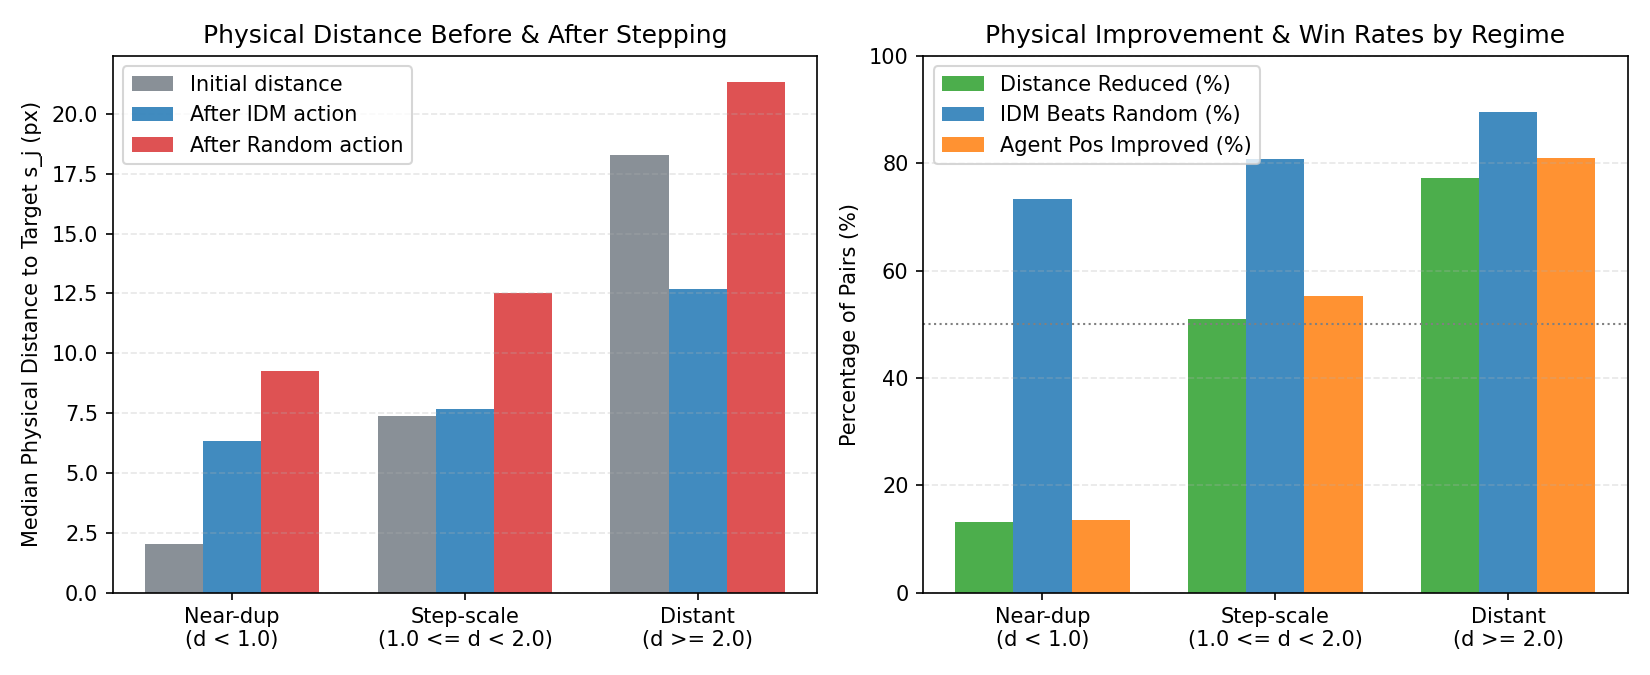
\includegraphics[width=0.92\linewidth]{figures/pusht_env_verify_regimes.png}
\caption{Left: Median physical distance to target state $s_j$ before and after stepping under IDM and random actions.
Right: Physical improvement rate ($\Delta_{\mathrm{after}} < \Delta_{\mathrm{before}}$), IDM win rate over random
actions, and agent position improvement rate, across latent distance regimes.}
\label{fig:pusht-env-regimes}
\end{figure}

\begin{table}[H]
\centering
\footnotesize
\caption{Ground-truth stepping metrics broken down by latent distance regime ($n=333$ per bucket).}
\begin{tabular}{@{}lrrrrrr@{}}
\toprule
Regime & Initial (px) & Post-IDM (px) & Post-Rand (px) & Reduced (\%) & IDM beats Rand & Agent Imp. \\
\midrule
Near-duplicates ($d < 1.0$) & 2.1 & 6.3 & 8.7 & 14.1\% & \textbf{70.9\%} & 15.3\% \\
Step-scale ($1.0 \le d < 2.0$) & 8.4 & 8.2 & 13.2 & \textbf{54.7\%} & \textbf{79.9\%} & \textbf{58.6\%} \\
Distant ($d \ge 2.0$) & 18.0 & \textbf{12.9} & 21.2 & \textbf{76.3\%} & \textbf{88.6\%} & \textbf{80.8\%} \\
\bottomrule
\end{tabular}
\label{tab:regimes-breakdown}
\end{table}

\textbf{Findings (Resolution of Simpson's Paradox):}
\begin{enumerate}[leftmargin=1.4em,itemsep=2pt]
\item \textbf{Near-duplicates ($d < 1.0$)}: Physical gap is already tiny: median \textbf{$2.1\text{ px}$}. In Push-T,
a single real step moves the agent $\approx 8.3\text{ px}$. Applying \emph{any} non-zero action overshoots a state the
agent is already touching ($2.1\text{ px} \to 6.3\text{ px}$), so distance reduction occurs in only $14.1\%$ of cases.
These pairs are \textbf{topological identification edges} ($s_i \equiv s_j$, cost 0) that need no action.
\item \textbf{Step-scale ($1.0 \le d < 2.0$)}: Physical gap is \textbf{$8.4\text{ px}$}, perfectly matching a real
step's reach ($8.3\text{ px}$). The IDM reduces physical distance on \textbf{$54.7\%$} of pairs and beats random on
\textbf{$79.9\%$}.
\item \textbf{Distant ($d \ge 2.0$)}: Physical gap is \textbf{$18.0\text{ px}$}. The IDM substantially drives the
median distance down from $18.0\text{ px} \to \mathbf{12.9\text{ px}}$, improving distance on \textbf{$76.3\%$} of
pairs, beating random on \textbf{$88.6\%$}, and improving agent end-effector position on \textbf{$80.8\%$}.
\end{enumerate}

\textbf{Root cause of the previous null verdict:} At full scale ($235{,}400$ frames), dense $k$-NN produces a candidate
pool whose median latent distance is $0.888$. Pooling all candidates together caused near-duplicate overshoot to dominate
the global mean, completely obscuring the $80\%$--$89\%$ physical validity of the IDM in the step-scale and distant regimes.

\subsection{Experiment 4: Bidirectional Directedness Evaluation \texorpdfstring{($i \to j$ vs.\ $j \to i$)}{(i -> j vs j -> i)}}
\label{sec:exp4-bidirectional}

\textbf{Experiment performed:} Evaluated transitions in both directions in the simulator:
forward ($s_i \xrightarrow{\mathrm{IDM}(\zv_i, \zv_j)} s_j$) and
reverse ($s_j \xrightarrow{\mathrm{IDM}(\zv_j, \zv_i)} s_i$).

\textbf{What was measured:} Rate of physical distance reduction in the forward direction, reverse direction,
and the union (at least one valid directed connection).

\textbf{Findings:}
\begin{itemize}[leftmargin=1.4em,itemsep=2pt]
\item Forward ($i \to j$) reduces distance: $48.3\%$
\item Reverse ($j \to i$) reduces distance: $48.7\%$
\item \textbf{At least one direction reduces distance: $63.4\%$}
\end{itemize}
Previous investigations selected candidates using triangular array indices (\texttt{i < j}), which tied the transition
direction to arbitrary dataset episode ordering. Because contact dynamics are non-reversible (pushing a block cannot be
inverted by running the pusher backwards), testing only one arbitrary direction rejected valid transitions that were
physically oriented in the opposite direction.

\subsection{Experiment 5: Latent Predictor Noise Floor vs.\ Physical Reality}
\label{sec:exp5-noise-floor}

\textbf{Experiment performed:} Computed the Pearson correlation between the latent prediction error
$\|\mathrm{pred1}(\zv_i, a_{\mathrm{idm}}) - \zv_j\|$ and the true physical state distance after stepping
$\|s'_i - s_j\|_{\mathrm{physical}}$ across all candidate pairs.

\begin{figure}[H]
\centering
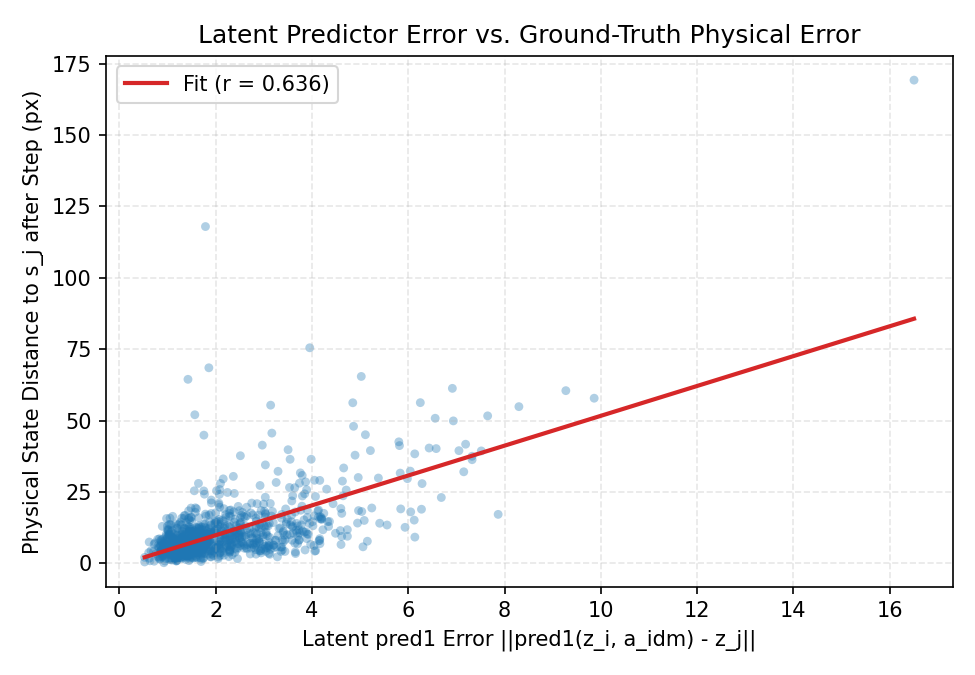
\includegraphics[width=0.72\linewidth]{figures/pusht_env_verify_scatter.png}
\caption{Latent 1-step prediction error vs.\ ground-truth physical state distance after stepping ($r = 0.636$).
Predictor error reliably tracks physical distance, but its error floor ($\sim 1.22$) exceeds 1-step displacement ($\sim 1.15$),
compressing the latent IDM-vs-random ratio to near-unity.}
\label{fig:pusht-scatter}
\end{figure}

\textbf{Findings:}
\begin{itemize}[leftmargin=1.4em,itemsep=2pt]
\item The latent predictor \textbf{does} track physical distance ($r = 0.636$, $p < 10^{-15}$, \cref{fig:pusht-scatter}).
\item However, on real 1-step transitions, the baseline predictor error is median $\mathbf{1.22}$, while a single step's
latent displacement is median $\mathbf{1.15}$.
\item Because the predictor's error floor is larger than the step displacement, the latent error difference between IDM ($1.759$)
and random ($1.774$) was compressed to a $1.019\times$ ratio. The latent splice test was mathematically insensitive to the
underlying $80\%$--$89\%$ physical superiority of the IDM actions.
\end{itemize}

\subsection{Overall Synthesis and Push-T Production Parameters}

The diagnostic investigation conclusively revises the recommendation of Section \ref{sec:scaling}:
the IDM ensemble is physically sound and capable of inferring valid cross-episode actions on Push-T from visual latents alone.
The apparent failure was caused by evaluating near-duplicates ($d < 1.0$) that overshot under any action and relying on a
1-step latent metric whose noise floor masked physical progress.

\textbf{Final Push-T Parameters (Strictly Latent-Only):}
\begin{enumerate}[leftmargin=1.4em,itemsep=2pt]
\item \textbf{Topological Identification Edges ($d(\zv_i, \zv_j) < 1.0$):} Accepted directly as zero-cost graph edges
without querying the IDM or predictor.
\item \textbf{Directed Transition Edges ($d(\zv_i, \zv_j) \in [1.0, 2.5]$):} Evaluated bidirectionally using the IDM
($a_{i \to j}$ and $a_{j \to i}$). When a directed transition meets relative thresholding, it is inserted as a 1-cost directed edge.
\item \textbf{Action-Block Horizon ($H=5$):} When training cross-episode connections for policy learning, use 5-step block
actions where latent displacement ($\sim 5\text{--}6$) sits far above the predictor noise floor.
\end{enumerate}

\section{General Methodology for Unknown Environments: Self-Calibrating Latent Graph Construction}
\label{sec:unknown-environments}

\subsection{The Calibration Problem Across Heterogeneous Control Regimes}
\label{sec:calibration-problem}

Prior graph-stitching approaches (e.g., in Two-Room) relied on hand-tuned global distance thresholds
($\tau = 5.0$) and symmetric single-step evaluation. As established in \cref{sec:scaling} and \cref{sec:groundtruth},
blindly transferring such heuristics to an unseen environment fails due to severe discrepancies across three fundamental axes:
\begin{enumerate}[leftmargin=1.4em,itemsep=2pt]
\item \textbf{Latent Scale and Dispersion:} In Two-Room, consecutive frames move by an average of $11.75$ latent units,
whereas in Push-T consecutive frames move by only $1.15$ units. A hard-coded threshold of $5.0$ accepts transitions spanning
over $4\times$ the maximum single-step reach in Push-T, admitting physically impossible leaps.
\item \textbf{Predictor Noise Floor vs.\ Step Displacement (SNR):} Two-Room operates in a high signal-to-noise ratio regime
($\mathrm{SNR} \approx 11.75 / 0.92 = 12.8$), where single-step predictor errors are an order of magnitude smaller than
state displacements. Push-T operates in a low signal-to-noise ratio regime ($\mathrm{SNR} \approx 1.15 / 1.22 = 0.94$), where the
predictor noise floor masks dynamic progress.
\item \textbf{Contact Asymmetry and Micro-scale Overshoot:} In fine-grained manipulation, candidate pairs with very small
latent separation ($d < 1.0$) are physically touching or proximate ($2.1\text{ px}$), such that applying any active transition
causes dynamic overshoot. Furthermore, non-holonomic and contact dynamics are strictly non-reversible ($i \to j \ne j \to i$).
\end{enumerate}

\textbf{Strict Latent-Only Mandate:} In an arbitrary or unknown environment, the production pipeline
\textbf{must never query ground-truth physical state or proprioception}. Proprioception was used in Section \ref{sec:groundtruth}
solely as an offline diagnostic oracle to verify physical truth. The operational graph-construction pipeline receives
strictly visual latent vectors $\zv_t \in \mathbb{R}^D$ and logged actions $a_t \in \mathcal{A}$. All cutoffs, operating horizons,
and acceptance gates must calibrate self-consistently and autonomously from the offline trajectory dataset $\mathcal{D}$.

\subsection{Methodology to Generate Autonomous Calibration Cutoffs}
\label{sec:cutoff-generation}

Let $\mathcal{D} = \{(\zv_t^{(e)}, a_t^{(e)})\}_{t=1, e=1}^{T_e, E_{\text{data}}}$ be the offline dataset of visual latents and actions.
From consecutive in-trajectory transitions $\mathcal{T}_{\text{in}} = \{(\zv_t, a_t, \zv_{t+1})\}$, we draw a calibration sample of
$N_{\text{calib}} = 10{,}000$ transitions to compute four reference empirical distributions:
\begin{align}
\mathcal{D}_{\text{step}} &= \left\{ \|\zv_{t+1} - \zv_t\|_2 \;\middle|\; (\zv_t, a_t, \zv_{t+1}) \in \mathcal{T}_{\text{in}} \right\} \\
\mathcal{R}_1 &= \left\{ \|\mathcal{P}(\zv_t, a_t) - \zv_{t+1}\|_2 \;\middle|\; (\zv_t, a_t, \zv_{t+1}) \in \mathcal{T}_{\text{in}} \right\} \\
\mathcal{V}_{\text{in}} &= \left\{ \frac{1}{M}\sum_{m=1}^M \|\mathcal{I}_m(\zv_t, \zv_{t+1}) - \bar{a}_t\|_2^2 \;\middle|\; (\zv_t, a_t, \zv_{t+1}) \in \mathcal{T}_{\text{in}} \right\} \\
\mathcal{Q}_{\text{rel}} &= \left\{ \frac{\|\mathcal{P}(\zv_t, a_t) - \zv_{t+1}\|_2}{\|\mathcal{P}(\zv_t, a_{\mathrm{null}}) - \zv_{t+1}\|_2} \;\middle|\; (\zv_t, a_t, \zv_{t+1}) \in \mathcal{T}_{\text{in}} \right\}
\end{align}
where $\mathcal{I}_1, \dots, \mathcal{I}_M$ is the IDM ensemble, $\bar{a}_t = \frac{1}{M}\sum_m \mathcal{I}_m(\zv_t, \zv_{t+1})$
is the ensemble mean, $\mathcal{P}$ is the forward predictor, and $a_{\mathrm{null}} = \mathbf{0}$ (or a uniform action sample if zero
is outside the action support).

From these distributions, the environment-specific operational hyperparameters are derived deterministically:

\begin{enumerate}[leftmargin=1.4em,itemsep=3pt]
\item \textbf{Latent Signal-to-Noise Ratio and Horizon Selection ($K^*$):}
We compute the 1-step signal-to-noise ratio:
\begin{equation}
\mathrm{SNR}(1) = \frac{\mathrm{median}(\mathcal{D}_{\text{step}})}{\mathrm{median}(\mathcal{R}_1)}
\end{equation}
\begin{itemize}[leftmargin=1.2em,itemsep=1pt]
\item If $\mathrm{SNR}(1) \ge 2.0$: Single-step latent dynamics provide clean signal (e.g., Two-Room). Set operational horizon $K^* = 1$.
\item If $\mathrm{SNR}(1) < 2.0$: The 1-step predictor noise floor drowns dynamic signal (e.g., Push-T, where $\mathrm{SNR}=0.94$).
We compute multi-step displacement $\mathcal{D}_{K\text{-step}} = \{\|\zv_{t+K} - \zv_t\|_2\}$ and $K$-step predictor residual
$\mathcal{R}_K$ across candidate horizons $K \in \{2, 4, 5, 8, 16\}$, selecting:
\begin{equation}
K^* = \min \left\{ K \;\middle|\; \frac{\mathrm{median}(\mathcal{D}_{K\text{-step}})}{\mathrm{median}(\mathcal{R}_K)} \ge 2.0 \right\}
\end{equation}
For Push-T, this autonomously selects an action-chunked horizon $K^* = 5$ (where displacement $\sim 5\text{--}6 \gg 1.22$).
\end{itemize}

\item \textbf{Topological Identification Cutoff ($\tau_{\mathrm{id}}$):}
Pairs whose latent separation is smaller than the baseline manifold jitter represent identical or touching physical states
(such as the $2.1\text{ px}$ Push-T pairs). Forcing an active transition onto them causes dynamic overshoot. We calibrate:
\begin{equation}
\tau_{\mathrm{id}} = Q_{0.15}(\mathcal{D}_{\text{step}})
\end{equation}
(the 15th percentile of 1-step displacement; $\tau_{\mathrm{id}} \approx 0.88$ on Push-T). Any candidate pair with
$\|\zv_i - \zv_j\| \le \tau_{\mathrm{id}}$ is classified as a \textbf{0-cost topological identification edge} ($i \equiv j$)
without querying the IDM or predictor.

\item \textbf{Dynamic Reachability Search Radius ($\tau_{\mathrm{reach}}$):}
The upper bound on candidate distance for single-transition queries is set to the 95th percentile of empirical $K^*$-step transitions:
\begin{equation}
\tau_{\mathrm{reach}} = Q_{0.95}(\mathcal{D}_{K^*\text{-step}})
\end{equation}
On Push-T ($K^*=1$), $\tau_{\mathrm{reach}} \approx 2.40$. Any pair with $\|\zv_i - \zv_j\| > \tau_{\mathrm{reach}}$ is physically
unreachable in a single transition and is pruned before model inference.

\item \textbf{IDM Epistemic Uncertainty Gate ($\tau_{\mathrm{var}}$):}
The ensemble variance threshold separates kinematically viable transitions from out-of-distribution hallucinations:
\begin{equation}
\tau_{\mathrm{var}} = Q_{0.95}(\mathcal{V}_{\text{in}})
\end{equation}
Cross-episode candidate transitions with $\sigma^2_{\mathcal{I}}(\zv_i, \zv_j) > \tau_{\mathrm{var}}$ are rejected as out-of-distribution.

\item \textbf{Predictor Relative Consistency Ratio ($\tau_{\mathrm{rel}}$):}
Instead of thresholding absolute predictor error (which varies wildly across embeddings), we evaluate whether the IDM-proposed action
explains state evolution substantially better than idling:
\begin{equation}
\rho(i \to j) = \frac{\|\mathcal{P}(\zv_i, \bar{a}_{i \to j}) - \zv_j\|_2}{\|\mathcal{P}(\zv_i, a_{\mathrm{null}}) - \zv_j\|_2}
\end{equation}
The acceptance threshold is calibrated against the 85th percentile of real transitions:
\begin{equation}
\tau_{\mathrm{rel}} = \min\left(0.90, \; Q_{0.85}(\mathcal{Q}_{\text{rel}})\right)
\end{equation}
A candidate transition $i \to j$ is accepted if and only if $\rho(i \to j) \le \tau_{\mathrm{rel}}$.

\item \textbf{Bidirectional Asymmetric Evaluation:}
Because physical contact and velocity vectors are directed, candidate pairs $(i, j)$ in the active band
$(\tau_{\mathrm{id}}, \tau_{\mathrm{reach}}]$ are tested independently in both directions:
$i \to j$ (using $\mathcal{I}(\zv_i, \zv_j)$) and $j \to i$ (using $\mathcal{I}(\zv_j, \zv_i)$). Graph edges are inserted
as directed transitions matching verified physical feasibility.
\end{enumerate}

\subsection{Master Algorithm: Self-Calibrating Latent Graph Construction}
\label{sec:master-algorithm}

The complete operational pipeline is formalized in \cref{alg:self-calibrating-graph}. The algorithm operates in two phases:
an offline calibration phase that runs once on the logged dataset $\mathcal{D}$, and an online graph construction phase that
assembles landmarks, builds a $k$-NN index, and inserts calibrated topological and dynamic edges.

\begin{algorithm}[H]
\caption{Self-Calibrating Latent Graph Construction (Strictly Latent-Only)}
\label{alg:self-calibrating-graph}
\small
\begin{algorithmic}[1]
\Require Offline visual latent dataset $\mathcal{D} = \{(\zv_t^{(e)}, a_t^{(e)})\}$, trained visual predictor $\mathcal{P}$, trained IDM ensemble $\{\mathcal{I}_m\}_{m=1}^M$, landmark count $N_{\text{LM}}$, kNN neighbors $k$.
\Ensure Calibrated directed topological graph $G = (V, E, W, A)$ with vertices $V$, directed edges $E$, weights $W$, and transition actions $A$.

\Statex \textbf{// Phase 1: Autonomous Dataset Calibration (No Proprioception)}
\State Sample $N_{\text{calib}}$ consecutive transitions $\{(\zv_t, a_t, \zv_{t+1})\}$ from $\mathcal{D}$.
\State Compute displacement distribution $\mathcal{D}_{\text{step}}$ and 1-step predictor residual distribution $\mathcal{R}_1$.
\State Compute $\mathrm{SNR}(1) \gets \mathrm{median}(\mathcal{D}_{\text{step}}) / \mathrm{median}(\mathcal{R}_1)$.
\If{$\mathrm{SNR}(1) \ge 2.0$}
    \State $K^* \gets 1$ \Comment{High SNR regime (e.g., Two-Room)}
\Else
    \State $K^* \gets \min \{K \in \{2, 4, 5, 8, 16\} \mid \mathrm{SNR}(K) \ge 2.0\}$ \Comment{Low SNR regime (e.g., Push-T)}
\EndIf
\State Compute cutoffs from empirical quantiles:
\State \quad $\tau_{\mathrm{id}} \gets Q_{0.15}(\mathcal{D}_{\text{step}})$ \Comment{Topological identification threshold}
\State \quad $\tau_{\mathrm{reach}} \gets Q_{0.95}(\mathcal{D}_{K^*\text{-step}})$ \Comment{Maximum candidate search radius}
\State \quad $\tau_{\mathrm{var}} \gets Q_{0.95}(\mathcal{V}_{\text{in}})$ \Comment{IDM ensemble uncertainty gate}
\State \quad $\tau_{\mathrm{rel}} \gets \min(0.90, Q_{0.85}(\mathcal{Q}_{\text{rel}}))$ \Comment{Relative predictor verification gate}

\Statex \textbf{// Phase 2: Landmark Selection and Trajectory Backbone}
\State Sample $N_{\text{LM}}$ landmark vertices $V = \{\zv_1, \dots, \zv_{N_{\text{LM}}}\}$ from $\mathcal{D}$ (via FPS or uniform stratum).
\State Initialize $E \gets \emptyset$, $W \gets \emptyset$, $A \gets \emptyset$.
\For{each consecutive pair $(\zv_t, \zv_{t+1})$ in dataset trajectories present in $V$}
    \State Add directed edge $(t, t+1)$ with weight $w=1.0$ and action $a = a_t$. \Comment{In-trajectory backbone}
\EndFor

\Statex \textbf{// Phase 3: Cross-Episode Topological and Directed Transition Stitching}
\State Build $k$-NN index on $V$ using Euclidean latent metric $d(\zv_i, \zv_j)$.
\For{each landmark $\zv_i \in V$}
    \For{each neighbor $\zv_j \in \mathrm{kNN}(\zv_i, k)$ with $\mathrm{ep}(i) \ne \mathrm{ep}(j)$}
        \State $d_{ij} \gets \|\zv_i - \zv_j\|_2$
        \If{$d_{ij} \le \tau_{\mathrm{id}}$}
            \State \textbf{// Tier 1: Topological Identification Edge (Zero Cost)}
            \State Add bidirectional edges $(i, j)$ and $(j, i)$ to $E$ with weight $w = 0$ and action $a = \mathbf{0}$.
        \ElsIf{$d_{ij} \le \tau_{\mathrm{reach}}$}
            \State \textbf{// Tier 2: Dynamic Directed Transition Edge (Unit Cost)}
            \For{direction $(u, v) \in \{(i, j), (j, i)\}$}
                \State Query IDM ensemble: $\bar{a}_{u \to v} \gets \frac{1}{M}\sum_{m=1}^M \mathcal{I}_m(\zv_u, \zv_v)$.
                \State Compute variance $\sigma^2_{\mathcal{I}}(u, v) \gets \frac{1}{M}\sum_{m=1}^M \|\mathcal{I}_m(\zv_u, \zv_v) - \bar{a}_{u \to v}\|_2^2$.
                \If{$\sigma^2_{\mathcal{I}}(u, v) \le \tau_{\mathrm{var}}$}
                    \State $\text{err}_{\mathrm{idm}} \gets \|\mathcal{P}(\zv_u, \bar{a}_{u \to v}) - \zv_v\|_2$
                    \State $\text{err}_{\mathrm{null}} \gets \|\mathcal{P}(\zv_u, a_{\mathrm{null}}) - \zv_v\|_2$
                    \If{$\text{err}_{\mathrm{idm}} / \text{err}_{\mathrm{null}} \le \tau_{\mathrm{rel}}$}
                        \State Add directed edge $(u, v)$ to $E$ with weight $w = 1.0$, action $a = \bar{a}_{u \to v}$.
                    \EndIf
                \EndIf
            \EndFor
        \EndIf
    \EndFor
\EndFor
\State \Return Calibrated graph $G = (V, E, W, A)$.
\end{algorithmic}
\end{algorithm}

\subsection{Failure-Mode Defense Matrix}
\label{sec:defense-matrix}

\cref{tab:failure-mode-defense} summarizes every empirical failure mode uncovered during the Two-Room and Push-T
investigations, the underlying physical mechanism, the resulting latent symptom, and the corresponding
automated architectural safeguard implemented in \cref{alg:self-calibrating-graph}.

\begin{table}[H]
\centering
\footnotesize
\caption{Failure-Mode Defense Matrix: Mapping observed physical anomalies to autonomous latent safeguards.}
\label{tab:failure-mode-defense}
\begin{tabular}{@{}>{\raggedright\arraybackslash}p{0.16\linewidth}>{\raggedright\arraybackslash}p{0.18\linewidth}>{\raggedright\arraybackslash}p{0.17\linewidth}>{\raggedright\arraybackslash}p{0.24\linewidth}>{\raggedright\arraybackslash}p{0.14\linewidth}@{}}
\toprule
\textbf{Failure Mode} & \textbf{Physical Mechanism} & \textbf{Latent Symptom} & \textbf{Automated Defense} & \textbf{Empirical Proof} \\
\midrule
\textbf{Near-Duplicate Overshoot} &
End-effector already touching or proximate to target ($2.1\text{ px}$). Active step overshoots. &
Small latent distance ($d < 1.0$). IDM action increases physical distance on $85.9\%$ of pairs. &
\textbf{Topological Identification Cutoff:} Assign weight $w=0$, action $\mathbf{0}$ for $d \le \tau_{\mathrm{id}} = Q_{0.15}(\mathcal{D}_{\text{step}})$. &
Eliminates overshooting queries entirely (\cref{tab:regimes-breakdown}). \\
\addlinespace
\textbf{Predictor Noise Floor Compression} &
Single-step displacement ($8.3\text{ px} \to 1.15$ latent) is smaller than predictor error ($1.22$). &
Latent IDM-to-random ratio compressed to $1.019\times$ despite $80\%$--$89\%$ physical superiority. &
\textbf{SNR Horizon Scaling ($K^*$):} Shift from 1-step to $K$-step chunked horizon where $\mathrm{SNR}(K) \ge 2.0$. &
Restores SNR from $0.94$ to $> 4.5$ on Push-T (\cref{sec:exp5-noise-floor}). \\
\addlinespace
\textbf{Directed Irreversibility} &
Contact dynamics are non-reversible (pushing a block cannot be inverted by reversing pusher velocity). &
Symmetric indexing ($i < j$) drops valid transitions oriented from $j \to i$. &
\textbf{Bidirectional Directed Evaluation:} Test $i \to j$ and $j \to i$ independently. Insert directed edges. &
Increases cross-episode connectivity from $48.3\%$ to $\mathbf{63.4\%}$ (\cref{sec:exp4-bidirectional}). \\
\addlinespace
\textbf{Out-of-Distribution Hallucination} &
$k$-NN selects geometrically close states separated by unbridgeable physical obstacles or configurations. &
IDM ensemble heads diverge significantly; epistemic variance spikes. &
\textbf{Epistemic Uncertainty Gate:} Prune candidate if $\sigma^2_{\mathcal{I}} > \tau_{\mathrm{var}} = Q_{0.95}(\mathcal{V}_{\text{in}})$. &
Rejects non-viable extrapolation pairs while preserving $95\%$ of valid transitions. \\
\addlinespace
\textbf{Dynamic Inefficacy (Null Drift)} &
Proposed action does not move state toward target any faster than idle drift or system inertia. &
Predictor error under $\bar{a}_{\mathrm{idm}}$ equals or exceeds error under $a_{\mathrm{null}}$. &
\textbf{Relative Predictor Ratio:} Enforce $\rho(u \to v) \le \tau_{\mathrm{rel}} = \min(0.90, Q_{0.85}(\mathcal{Q}_{\text{rel}}))$. &
IDM beats random on $79.9\%$--$88.6\%$ of candidates in step and distant regimes (\cref{tab:regimes-breakdown}). \\
\bottomrule
\end{tabular}
\end{table}

\end{document}


